\documentclass[blue]{elegantnote}

\author{}
\email{}
\zhtitle{电机学(下)}
\entitle{Electric Machine}
\version{1.00}
\myquote{Victory won\rq t come to us unless we go to it.}
\logo{logo.pdf}
\cover{cover.pdf}

%green color
   \definecolor{main1}{RGB}{210,168,75}
   \definecolor{seco1}{RGB}{9,80,3}
   \definecolor{thid1}{RGB}{0,175,152}
%cyan color
   \definecolor{main2}{RGB}{239,126,30}
   \definecolor{seco2}{RGB}{0,175,152}
   \definecolor{thid2}{RGB}{236,74,53}
%cyan color
   \definecolor{main3}{RGB}{127,191,51}
   \definecolor{seco3}{RGB}{0,145,215}
   \definecolor{thid3}{RGB}{180,27,131}

\usepackage{makecell}
\usepackage{lipsum}
\usepackage{caption}
\usepackage{subfigure}
\usepackage{ upgreek }
\usepackage{ textcomp }
\usepackage{ gensymb }
\usepackage{amsmath}
\usepackage{indentfirst}  % 用于首行缩进


\setlength{\parindent}{2em}   %缩进2字符
%如果有一个段落你不想首行缩进, 在段落前使用命令 \noindent.
%同样的, 你要保证这一段是首行缩进, 使用命令 \indent

% 用于插入转换为Tikz的matlab图形的宏包
 \usepackage{pgfplots}
\pgfplotsset{compat=newest}
%% the following commands are needed for some matlab2tikz features
\usetikzlibrary{plotmarks}
\usetikzlibrary{arrows.meta}
\usepgfplotslibrary{patchplots}
\usepackage{grffile}


 \begin{document}
\maketitle
\tableofcontents
\chapter{三相异步电动机的运行原理(9)}
异步电机和变压器都属于单边励磁的电机(转子侧的电流是由感应产生的)。从电磁关系看,定子绕组相当于变压器的一次绕组,转子绕组相当于变压器的二次绕组。异步电机三相定、转子绕组对称,正常对称运行时,各相发生的电磁过程完全相同。因此,可以把分析变压器的理论用到分析异步电机中。

\begin{figure}[!hbtp]
	\centering
	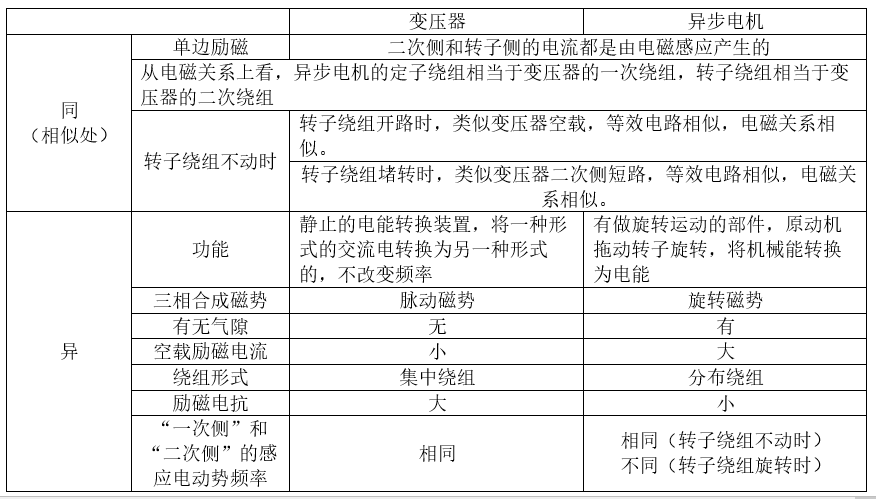
\includegraphics[width=\textwidth,height=0.6\textwidth]{conclusion_9.png}
	\caption{异步电动机和变压器异同}
\end{figure}

\newpage
\section{转子不动}

\subsection{转子绕组开路}
{\color{thid}转子开路时,无$\dot I_2$,相当于变压器开路}
\begin{enumerate}
	\item 基波磁动势:
	\newline 磁动势{\color{blue}只由定子产生},为旋转磁动势,{\color{blue}以同步转速$n_1=\frac{60f_1}{p}$旋转}
	\item 主磁通和定子漏磁通:
	\item 感应电动势:
	\newline{\color{blue}$E_1$和$E_{20}$频率相同},都等于主磁通$\dot\phi_m$频率{\color{blue}$f_1$}
	\item 电压平衡方程:
	\newline$\dot{U_1}=-\dot{E_1}+\dot{I_{\color{blue}0}}(r_1+jx_1)=-\dot{E_1}+\dot{I_{\color{blue}0}}Z_1$
	\newline $\dot{U_2}=\dot{E_{2{\color{blue}0}}}$
	\item 等效电路:
	\newline $\dot E_1$用励磁电流$\dot I_0$在励磁阻抗$Z_m$上的压降表示: $\dot E_1=-\dot{I_0}Z_m$
	\newline 定子绕组一相平衡方程为: $\dot U_1=\dot{I_0}(Z_1+Z_m)$
\end{enumerate}
\begin{figure}[!hbtp]
	\centering
	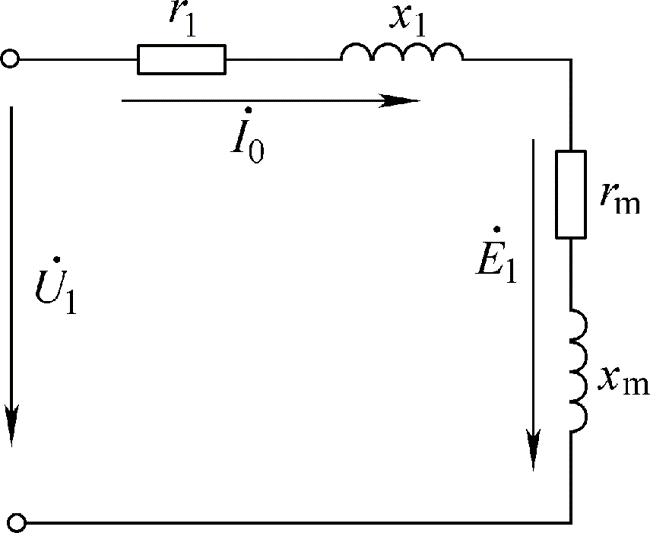
\includegraphics[width=0.3\textwidth,height=0.2\textwidth]{zhuanzi_kailu.png}
	\caption{转子开路的等效电路\label{figur:zhuanzi_kailu}}
\end{figure}
\subsection{转子绕组堵转}
堵转:转子绕组三相绕组{\color{blue}短路},且转子{\color{blue}堵住不转}。
\newline{\color{thid}转子堵转时,有$\dot I_2$,相当于变压器短路}
\begin{enumerate}
	\item 基波磁动势:
	\newline 由{\color{blue}定子}和{\color{blue}转子}产生,都为旋转磁动势,相对静止,{\color{blue}以同步转速$n_1=\frac{60f_1}{p}$旋转}
	\item 感应电动势:
	\newline{\color{blue}$E_1$和$E_{20}$频率相同},都等于主磁通$\dot\phi_m$频率{\color{blue}$f_1$}
	\item 电压平衡方程:
	\newline$\dot{U_1}=-\dot{E_1}+\dot{I_1}(r_1+jx_1)=-\dot{E_1}+\dot{I_1}Z_1$
	\newline $\dot E_{2{\color{blue}0}}=\dot{I_2}(r_2+jx_{2{\color{blue}0}})=\dot I_2Z_{2{\color{blue}0}}$
	\item 磁动势平衡: $\dot F_1+\dot F_2=\dot F_0$
	\item 转子绕组的折算:\\
	\begin{table}[h]
		\centering
		\begin{tabular}{|c|c|c|}
			\hline 
			\phantom{折算前} &折算前 &折算后  \\ \hline
			相数 & $m_2$ & $m_1$ \\ \hline
			匝数 & $N_2$ & $N_1$ \\ \hline
			绕组系数 & $k_{w2}$  &  $k_{w1}$ \\ \hline
		\end{tabular}
	\end{table}
	\begin{note}
		(1)电流的折算:折算前后磁动势$\dot{F_2}$不变
		\newline \indent(2)电动势及电压的折算:折算前后电磁功率不变$(m_1{E_2}^{'}{I_2}^{'}=m_1E_2I_2)$
		\newline \indent(3)阻抗的折算:电阻(折算前后铜耗不变,$(m_1{r_2}^{'}{I_2}^{'2}=m_1r_2{I_2}^2)$ )
		\newline 电抗(折算前后功率因数不变,$tan\theta_2=\frac{x_2}{r_2}=\frac{{x_2}^{'}}{{r_2}^{'}}$)
	\end{note}
	\item 等效电路:
	\newline $\dot E_1$用励磁电流$\dot I_0$在励磁阻抗$Z_m$上的压降表示: $\dot E_1=-\dot{I_0}Z_m$
	\newline 定子绕组一相平衡方程为: $\dot U_1=\dot{I_0}(Z_1+Z_m)$
	\begin{figure}[!hbtp]
		\centering
		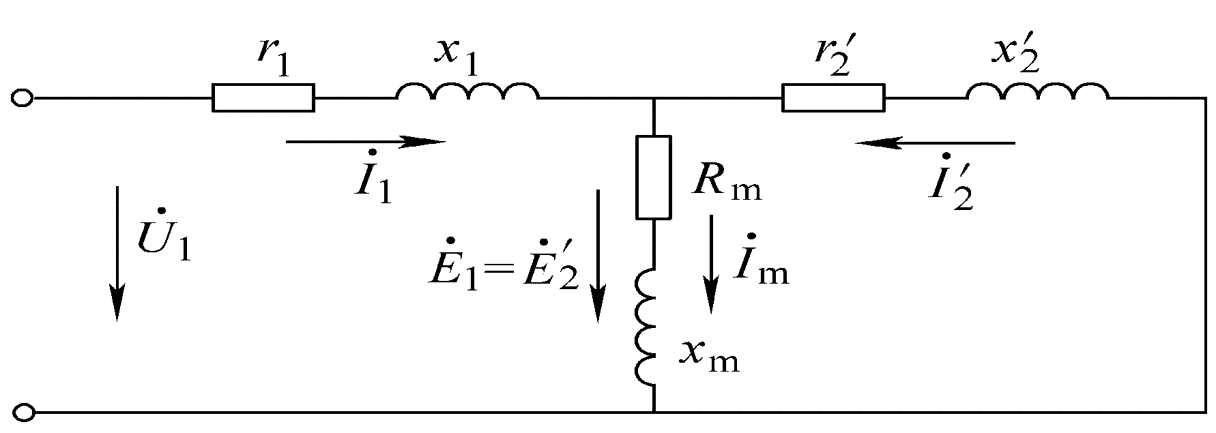
\includegraphics[width=0.4\textwidth,height=0.2\textwidth]{zhuanzi_duzhuan.png}
		\caption{转子堵转的等效电路\label{figur:zhuanzi_duzhuan}}
	\end{figure}
\end{enumerate}
\section{转子旋转}
定子回路的情况不变,{\color{thid}只有\underline{转子}绕组中\underline{感应电动势}的频率、大小及\underline{漏抗}都发生变化}
\\  转差率:$s=\frac{n_1-n}{n_1}$ ($n_1$为同步转速,$n$为转子转速) \\
\begin{enumerate}
	\item 电磁关系:
	\\$\dot F_1$和$\dot F_2$相对静止($\dot F_2$相对于转子的转速为$n_1-n$,相对于定子转速为$n_1$ )\\
	\begin{note}
		转子虽然旋转,但转矩固定,所以,定子磁动势和转子磁动势相对静止
	\end{note}
	\begin{table}[h]
		\centering
		\begin{tabular}{|c|c|c|}
			\hline
			\phantom{转子}  & 转子  & 定子  \\ \hline
			感应电动势的频率   &  $f_1$   &  $f_2=sf_1$   \\ \hline
			漏阻抗           &    与$n$无关   & $x_{2s}$与$n$有关  \\ \hline
			磁动势频率(相对定子)   &     $n_1$   &    $n_1$   \\ \hline
			磁动势频率({\color{blue}相对转子})   &  $n_1-n=sn_1s$      &    $n_1-n=sn_1$   \\ \hline
		\end{tabular}
	\end{table}
	\item 频率折算:{\color{thid}用一个静止的具有电阻为$r_2/s$的等效不动转子去代替电阻为$r_2$的实际旋转转子,等效转子与实际转子具有相同的转子磁动势。}
	\begin{newproof}
		\\转子转动后,转子电流有:
		$$\dot I_2=\frac{\dot E_2}{r_2+jx_{2s}}=\frac{s\dot{E_{20}}}{r_2+jsx_{20}}=
		\frac{\dot{E_{20}}}{\frac{r_2}{s}+jx_{20}}$$
	\end{newproof}
	\begin{table}[!h]
		\centering
		\begin{tabular}{|c|c|c|}
			\hline 
			\phantom{折算前} &折算前 &折算后  \\ \hline
			转子电流  &  $\dot I_2(f_2)$   &  $\dot I_{20}(f_1)$  \\ \hline
			电动势   &  $\dot E_2=s\dot E_{20}$   &    $\dot E_{20}$  \\  \hline
			电抗     &    $x_2=s x_{20}$    &   $x_{20}$   \\ \hline
			电阻  &   $r_2$    &    $\frac{r_2}{s}$    \\   \hline
		\end{tabular}
	\end{table}
	\begin{note}
		\\$\frac{r_2}{s}\quad=\quad \phantom{aaaa}r_2\phantom{aaaaaaaa}+\phantom{aaaaaa}{\color{blue}\frac{1-s}{s}r_2}$
		\\$\frac{r_2}{s}\quad=\quad$转子本身电阻\phantom{aaa}+\phantom{aaaaa}{\color{blue}附加电阻}
		\\{\color{blue}附加电阻物理意义:异步电动机轴上总机械功率的等效电阻}
	\end{note}
	异步电机基本方程:
	$$ \dot U_1=-\dot E_1+\dot I_1(r_1+jx_1) $$
	$$  0=\dot E_2-\dot I2^{'}(r_2^{'}/s+jx_2^{'}) $$
	$$  \dot I_1 = \dot I_0+(-\dot I_2^{'})  $$
	$$   \dot E_1 = \dot E_2^{'}=-\dot I_0(r_,+jx_m)  $$
	\item 等效电路:
	\begin{figure}[!hbtp]
		\centering
		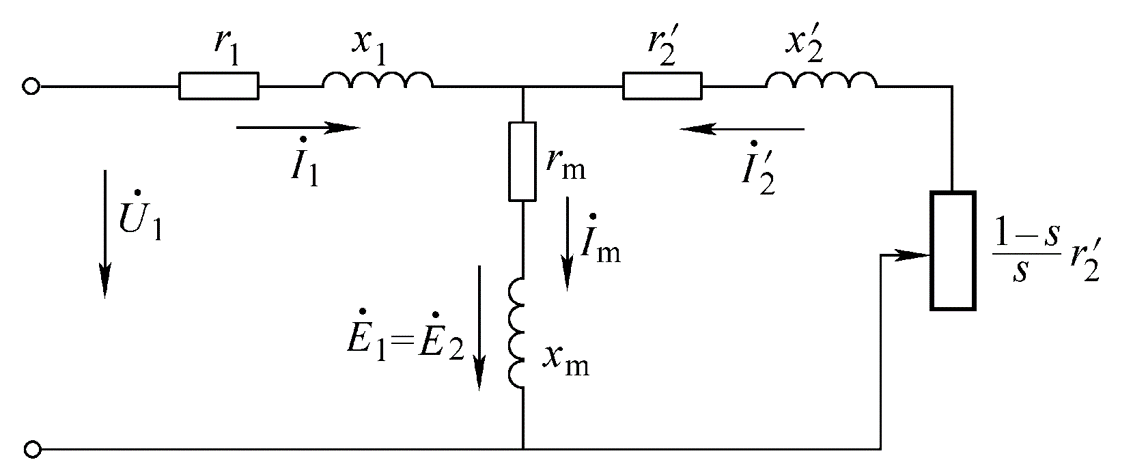
\includegraphics[width=0.5\textwidth,height=0.2\textwidth]{zhuanzi_xz.png}
		\caption{转子旋转的等效电路\label{figur:zhuanzi_xz}}
	\end{figure}
	\begin{table}[!htbp]
		\centering
		\begin{tabular}{|c|c|c|c|c|c|c|}
			\hline
			& $s$ & $n$ & $\frac{1-s}{s}r_2^{'}$  &  $I_2^{'}$   &说明 & 功率因数               
			\\ \hline 轻载  & $\approx 0$ & $\approx n_1$ & $\approx\infty$ & $\approx 0$ & 相当于转子侧开路 &  定子侧很低
			\\ \hline 起动   &  $1$ & $0$  &  $0$ & 很大 &  相当于转子侧短路 & 定子侧和转子侧都低
			\\ \hline 额定负载  & $0.02\sim0.06$ & &  & 阻性,不大 &  & 定子侧和转子侧都高
			\\ \hline        
		\end{tabular}
	\end{table}
	\begin{note}
		\\(1)轻载时,转子电流$\approx 0$,,定子电流几乎全是励磁电流,定子功率因数很低,但$Z_m$和$Z_2^{'}$相差没有变压器那么大。
		\\(2)启动时,相当于转子侧短路,但一般$x_2^{'}\gg r_2^{'}$,所以转子侧电流为感性。
		\\(3)额定负载时,转子电流不大,同时由于{\color{main}转子电流频率很低},$r_2^{'}\gg x_2^{'}$,所以转子侧电流为阻性,功率因数高。
	\end{note}
	
	\newpage
	\item 向量图:
	异步电机总为{\color{main}感性负载},电动机所需的励磁电流$\uparrow$,或定、转子漏抗$\uparrow$$\quad \Rightarrow$电动机功率因数$\downarrow$\\
	\begin{figure}[!hbtp]
		\centering
		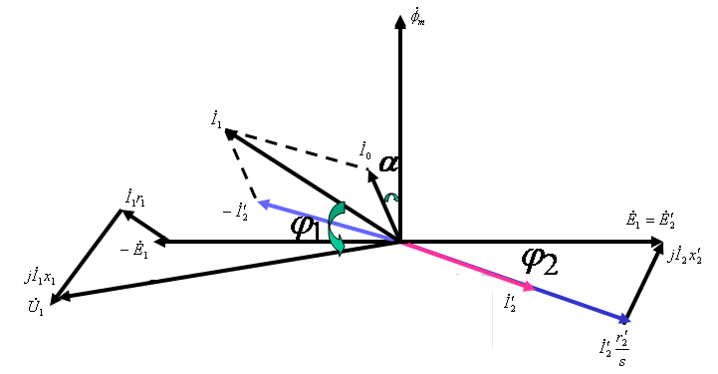
\includegraphics[width=0.8\textwidth,height=0.5\textwidth]{yibu_xiangl.png}
		\caption{异步电动机的向量图\label{figur:yibu_xiangl}}
	\end{figure}
	
	\item $T$型等效电路的简化:
	\begin{figure}[hb]
		\centering
		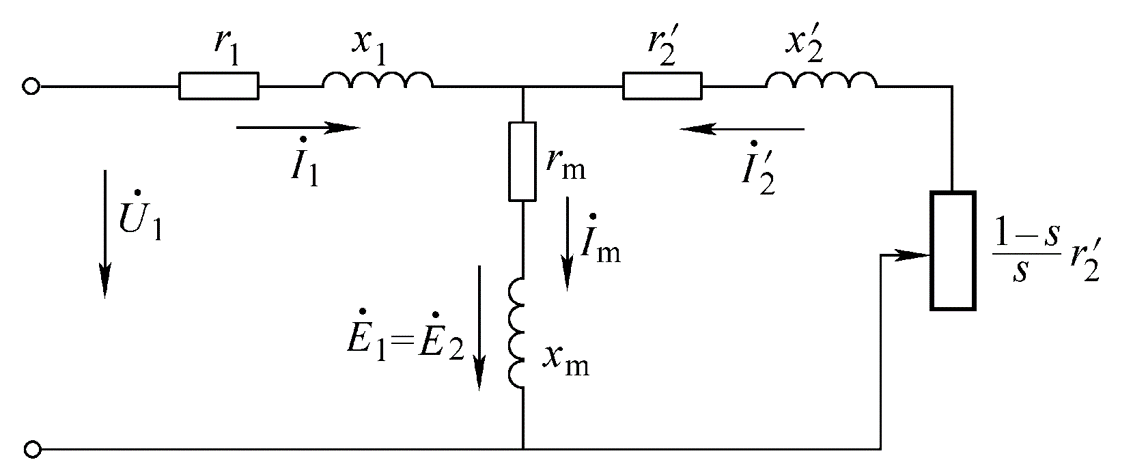
\includegraphics[width=0.5\textwidth,height=0.2\textwidth]{zhuanzi_xz.png}
		\caption{$T$型等效电路\label{figur:T_dx}}
	\end{figure}
	\begin{newproof}
		从$T$型等效电路可直接求得:$$\dot I_1=\frac{\dot U_1}{Z_1+Z_2^{'}//Z_m}$$    
		$$\dot I_2^{'}=-\dot I_1\frac{Z_m}{Z_m+Z_2^{'}}=-\frac{\dot U_1}{Z_1+\dot C_1Z_2^{'}}$$  
		$$\dot I_0 = \dot I_1\frac{Z_2^{'}}{Z_m+Z_2^{'}}=\frac{\dot U_1}{Z_m}\frac{1}{\dot C_1+\frac{Z_1}{Z_2^{'}}}$$
		其中修正系数(一般情况下,{\color{blue}电抗$\gg$电阻})
		$$\dot C_1=1+\frac{Z_1}{Z_m}\approx1+\frac{x_1}{x_m}$$ 
	\end{newproof}
	
	\begin{itemize}
		\item $\Gamma$型等效电路\\
		电动机正常工作时,{\color{blue}$\left|  Z_1 \right| \ll \left| Z_2^{'}\right|$},所以近似取$Z_1/Z_2^{'}\approx 0$,所以$$\dot I_0\approx\frac{\dot U_1}{Z_m+Z_1}$$
		\\ 又因为$$\dot C_1(r_m+jx_m)=(1+\frac{Z_1}{Z_m})Z_m=Z_m+Z_1$$ $$\dot I_2^{'}=-\frac{\dot U_1}{Z_1+\dot C_1Z_2^{'}}$$  $$\dot I_1 = \dot I_0-\dot I_2^{'}$$
		所以,有
		\begin{figure}[!hbtp]
			\centering
			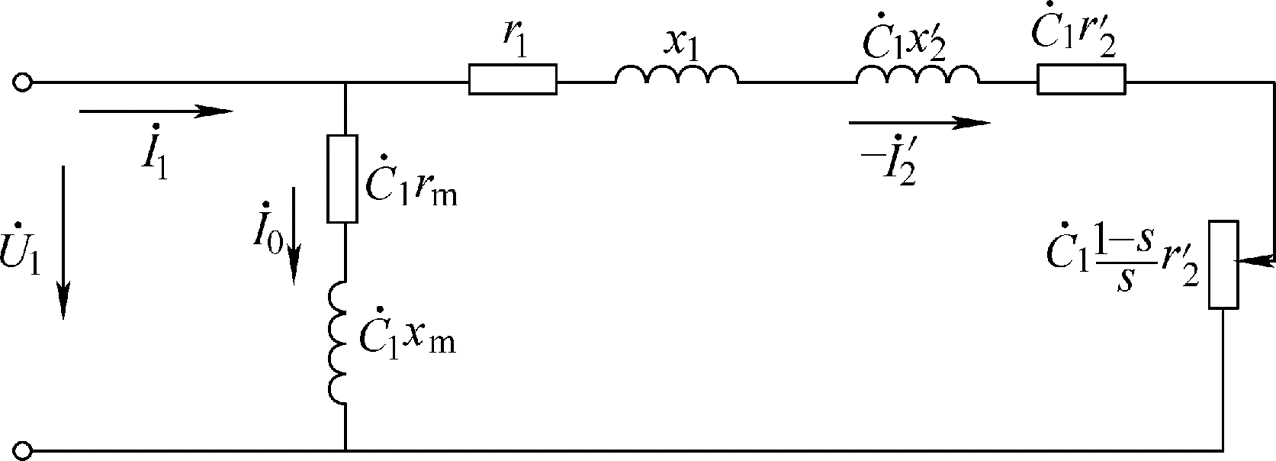
\includegraphics[width=0.5\textwidth,height=0.2\textwidth]{d_L_dx.png}
			\caption{$\Gamma$型等效电路\label{figur:d_L_dx}}
		\end{figure}
		
		\item 简化等效电路
		取$\dot C_1=1$,有
		\begin{figure}[!hbtp]
			\centering
			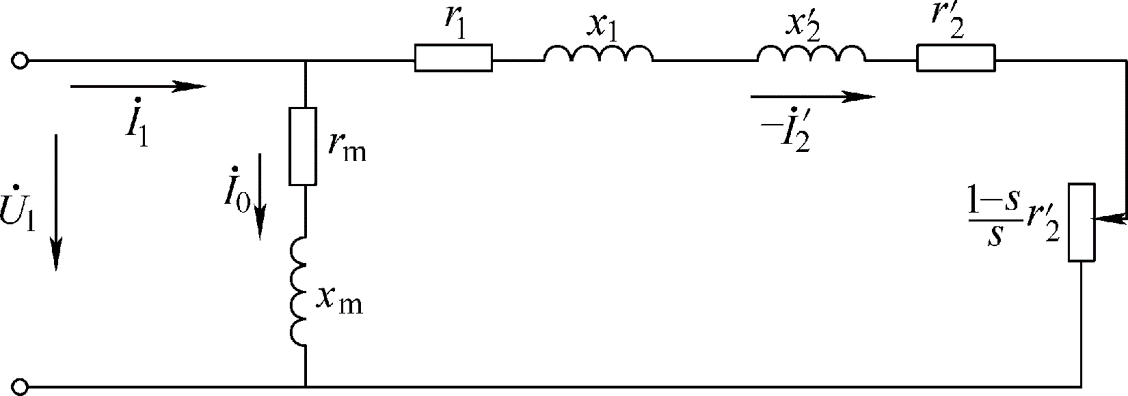
\includegraphics[width=0.5\textwidth,height=0.2\textwidth]{jh_dx.png}
			\caption{简化等效等效电路\label{figur:jh_dx}}
		\end{figure}
	\end{itemize}
\end{enumerate}

\chapter{三相异步电动机的功率、转矩与性能(10)}
\section{功率与转矩平衡}
\subsection{功率平衡}
\begin{enumerate}
	\item 从交流电源输入的有功功率:$P_1=3U_1I_1cos\phi_1$
	\begin{note}
		$U_1$和$I_1$为定子相电压和相电流,$cos\phi_1$为定子功率因数。
	\end{note}
	\item 定子铜耗:$p_{Cu1}=3I_1^2r_1$
	\item 异步电动机铁耗(主要指定子铁耗):$p_{Fe}=p_{Fe1}=3I_0^2r_m$
	\begin{note}
		三相异步电动机正常运行时,转子转速接近同步转速,{\color{main}转差率小,所以转子电动势频率很低}(这里是磁场频率低,导致铁耗小),大约为$1\sim3Hz$;转子铁芯和定子铁芯一样是由{\color{main}硅钢片叠成的}。所以,{\color{thid}一般忽略不计转子铁芯的铁耗。}
	\end{note}
	\item 电磁功率(通过气隙磁场,从定子传到转子的功率):$P_{em}=P_1-p_{Cu}-p_{Fe}$
	\\根据$T$型等效电路,$P_{em}=3{E_2}^{'}{I_2}^{'}cos\phi_2=3{I_2}^{'2}\frac{r_2^{'}}{s}=3{I_2}^{'2}(r_2^{'}+\frac{1-s}{s}r_2^{'})=p_{Cu2}+P_m$
	\begin{note}
		$p_{Cu2}$为转子绕组铜耗(转差功率,转差率越大,$p_{Cu2}$越大),$P_m=3I_2^{'2}\frac{1-s}{s}r_2^{'}$为附加电阻的损耗(总机械功率)。整理得:$P_{em}:P_m:p_{Cu2}=1:(1-s):s$
	\end{note}
	\item 机械损耗:$p_m$,附加损耗:$p_s$
	\begin{note}
		机械损耗:轴承以及风阻等摩擦转矩,附加损耗(一般由经验估算):由定转子开槽和定转子磁动势中的谐波磁动势等引起
	\end{note}
	\item 转子上真正输出的机械功率:$P_2=P_m-p_m-p_s$  
	\begin{figure}[!hbtp]
		\centering
		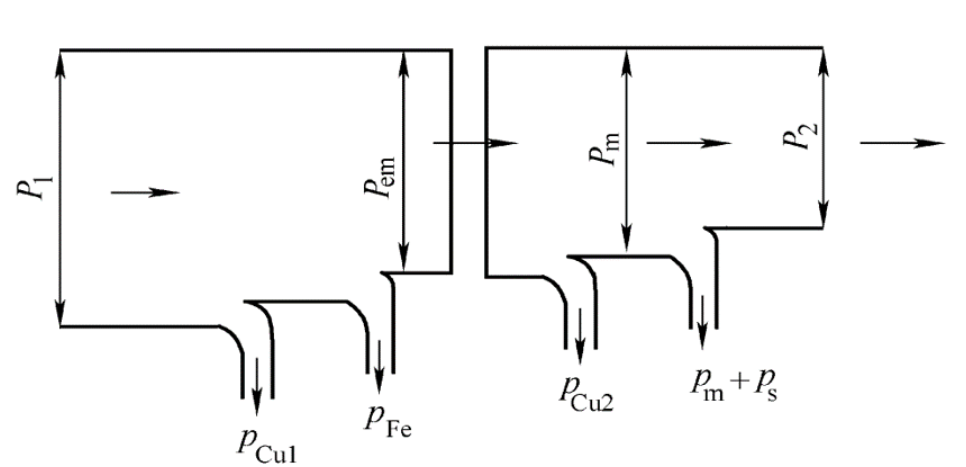
\includegraphics[width=0.7\textwidth,height=0.3\textwidth]{yibu_gllc.png}
		\caption{异步电动机的功率流程\label{figur:yibu_gonglv}}
	\end{figure}
\end{enumerate}

\newpage
\subsection{转矩平衡}
\underline{转矩平衡方程:$T_2=T-T_0$}
\\其中,$\Omega$为转子机械角速度,$\Omega=\frac{2\pi n}{60}$;$T_2$为输出转矩,$T_2=\frac{P_2}{\Omega}$;$T$为电磁转矩,$T=\frac{P_m}{\Omega}$;$T_0$为空载转矩(机械损耗$p_m$和附加损耗$p_s$对应的阻力转矩),$T_0=\frac{p_m+p_s}{\Omega}$
\\
\begin{newproof}
	$$P_2=P_m-p_m-p_s\Rightarrow \boxed{\frac{P_2}{\Omega}=\frac{P_m}{\Omega}-\frac{p_m+p_s}{\Omega}}$$
\end{newproof}
\begin{note}
	$$\boxed{T=\frac{P_m}{\Omega}}=\frac{P_{em}}{\Omega}(1-s)=\frac{P_{em}}{2\pi n/60}(1-s)=\frac{P_{em}}{2\pi n_1/60}(1-s)\boxed{=\frac{P_{em}}{\Omega_1}}$$
	($\Omega_1$为旋转磁场的同步角速度,$\Omega_1=\frac{2\pi n_1}{60}=\frac{2\pi}{60}\frac{60f_1}{p}=\frac{2\pi f_1}{p}=\frac{\omega_1}{p}$)
\end{note}

\section{电磁转矩及机械特性}
\subsection{电磁转矩}
\begin{enumerate}
	\item 物理表达式:
	$\boxed{T=C_T\Phi_m{I_2^{'}cos\phi_2}}$
	\begin{note}
		$$P_{em}=m_1E_2^{'}I_2^{'}cos\phi_2$$
		$$\Rightarrow T=\frac{P_{em}}{\Omega_1}=\frac{P_{em}}{\omega_1/p}=\frac{P_{em}}{2\pi f_1/p}=m_1\frac{p}{2\pi f_1}\times 4.44f_1N_1k_{w1}\Phi_mI_2^{'}cos\phi_2=C_T\Phi_m{\color{blue}\boxed{I_2^{'}cos\phi_2}}$$
		$m_1$—定子绕组相数;$C_T=\frac{m_1p}{\sqrt{2}}N_1k_{w1}$—转矩系数{\color{thid}(制造好的电机,为常数)};{\color{blue}$\Uparrow$}
		\\{\rightline{{\color{blue}转子电流有功分量}}}
	\end{note}
	\item 参数表达式:$ \boxed{ T=\frac{pm_1}{2\pi f_1}U_1^{2}\frac{\frac{r_2^{'}}{s}}{({\frac{r_2^{'}}{s}})^2+x_k^{2}}}$
	\begin{note}
		$$P_{em}m_1I_2^{'2}\frac{r_2^{'}}{s}$$
		(从$\tau$型等效电路得出)
		$$\Rightarrow T=\frac{pm_1}{2\pi f_1}U_1^{2}\frac{\frac{r_2^{'}}{s}}{({\frac{r_2^{'}}{s}})^2+x_k^{2}}$$
		$x_k$—异步电动机的短路电抗($x_k=x_1+x_2^{'}$)
	\end{note}
\end{enumerate}
\subsection{机械特性——$T=f(s)$曲线}
$$T=\frac{pm_1}{2\pi f_1}U_1^{2}\frac{\frac{r_2^{'}}{s}}{(\frac{r_2^{'}}{s})^{2}+x_k^{2}}$$
固有机械特性(定转子回路不串入任何电路元件时):
\begin{figure}[!hbtp]
	\centering
	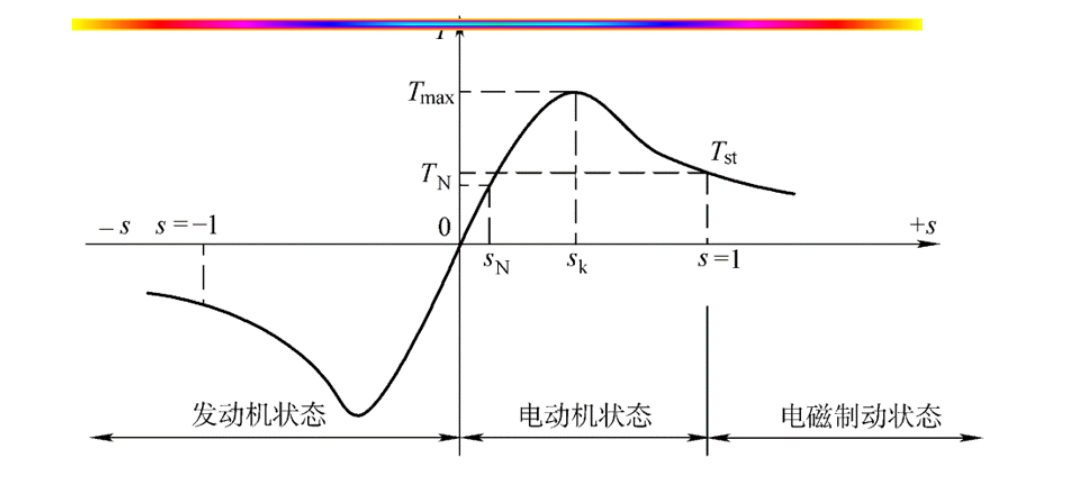
\includegraphics[width=0.9\textwidth,height= 0.5 \textwidth]{gyjx.png}
	\caption{固有机械特性\label{figur:gyjx}}
\end{figure}
\\特殊点:
\begin{table}[!htb]
	\begin{tabular}{|c|c|c|c|}
		\hline
		&   额定转矩$T_N$ &   最大电磁转矩$T_{max}$    &    启动转矩$T_{st}$    \\ \hline
		运行条件 &  额定负载       &   T最大时($dT/ds=0)$      &      	启动时   \\ \hline
		转速$n$  &  额定转速$n_N$  &                            &     0        \\ \hline
		转差率$s$&   额定转差率$s_N$          &  (临界转差率){\color{blue} $s_k=\frac{r_2^{'}}{x_k}$}&   1  \\ \hline           
	\end{tabular}
	\centering
\end{table} 
\\
\begin{enumerate}
	\item 额定转矩: $$T_N=\frac{P_N}{\Omega_N}=\frac{P_N}{2\pi n_N/60}=9550\frac{P_N}{n_N}$$
	\item    最大转矩: $$T_{max}=\frac{m_1p}{\omega_1}U_1^{2}\frac{1}{2x_k}$$
	\item 启动转矩:($s=1$代入)
	$$T=\frac{pm_1}{2\pi f_1}U_1^{2}\frac{r_2^{'}}{r_2^{'2}+x_k^{2}}$$
	要使启动时有最大转矩,转子回路串入电阻,使临界转差率$s_k=\frac{r_2^{'}}{x_k}=1$
	\item 过载能力:($K_m$越大,承受短时过载能力越低)
	$$K_m=\frac{T_{max}}{T_N}$$
	\item 启动转矩倍数:($T_{st}$越大,电机启动越容易)
	$$K_{st}=\frac{T_{st}}{T_N}$$
\end{enumerate}
\subsection{稳定运行条件}
\begin{itemize}
	\item 恒转矩负载(转速$n$变化时,负载转矩$T_L$保持恒定):
	$$\frac{dT}{ds}>0(\frac{dT}{dn}<0)$$
	\item 离心式负载(转速$n$上升时,负载转矩$T_L$上升):
	$$\frac{dT}{ds}>\frac{dT_L}{ds}(\frac{dT}{dn}<\frac{dT_L}{dn})$$
\end{itemize}
\subsection{工作特性}
{\color{thid}前提:额定电压,额定频率}\\
{\color{blue}要点:稳定运行时,负载不变$\Rightarrow$电机输出的驱动转矩不变}
\begin{figure}[!hbtp]
	\centering
	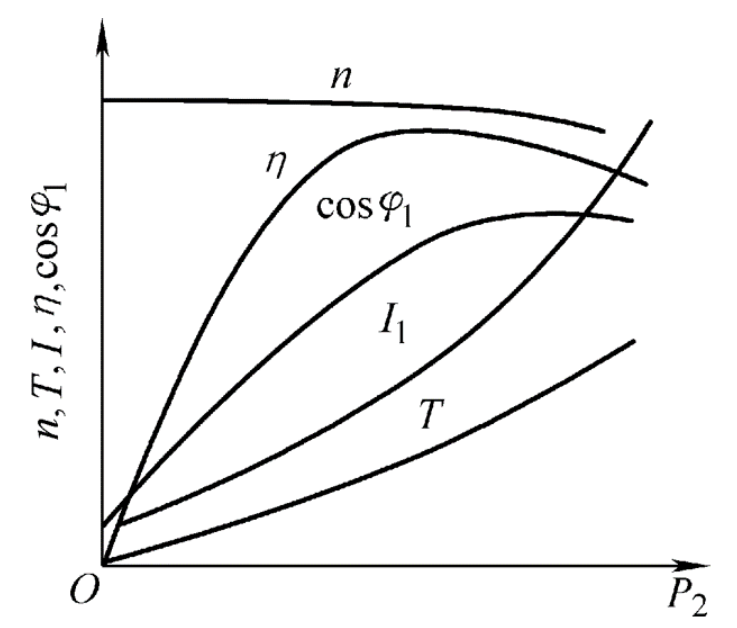
\includegraphics[width=0.5\textwidth,height= 0.4 \textwidth]{yb_gztx.png}
	\caption{异步电动机工作特性\label{figur:yb_gztx}}
\end{figure}
\begin{enumerate}
	\item 转速调整曲线$n=f(P_2)$或$s=f(P_2)$
	
	\item 电磁转矩特性$T=f(P_2)$
	
	\item 功率因数特性$cos\phi_1=f(P_2)$
	
	\item 定子电流特性$I_1=f(P_2)$
	
	\item 效率特性曲线$\eta=f(P_2)$
	
\end{enumerate}
\subsection{参数测定}
\begin{enumerate}
	\item 空载试验{\color{thid}(不带负载,不是开路)}
	$$P_0=p_{Cu1}+p_1+p_m$$
	{\color{thid}定子铜耗$p_{Cu1}$不能忽略(异步电机空载电流较变压器大)}
	$$P_{Fe}=p_0-3I_{0\Phi}^2r_1-p_m$$
	{\color{thid}转速基本不变时,认为机械损耗为常数}将$P_0^{'}=f(U_0^{2})$曲线,延长至与纵轴相交,相交点(0,$p_m$)\\
	$$r_m=\frac{p_{Fe}}{3I_{0\Phi}^2}$$
	{\color{thid}额定电压下空载,转速接近同步转速,即$s\approx 0$},转子侧相当于开路
	$$Z_0=(r_1+r_m)+j(x_1+x_m)$$
	$$x_0=\sqrt{Z_0^2-r_0^2}$$
	\item 短路试验{\color{thid}(堵转)}
	$$r_k=\frac{P_k}{3I_{k\Phi^2}}$$
	$$Z_k=\frac{U_{k\Phi}}{I_{k\Phi}}$$
	$$x_k=\sqrt{Z_k^2-r_k^2}$$
	{\color{blue}大、中型电机:$x_1=x_2^{'}=x_k/2$\\
		小型电机;用电桥测量定子直流电阻$r_1$}
\end{enumerate}


\chapter{三相异步电动机的起动、调速和制动(11)}
\section{起动}
\subsection{三相笼型异步电动机的起动}
\begin{enumerate}
	\item 全压起动(直接起动)
	\begin{itemize}
		\item[-] 缺点:{\color{thid}启动电流大},过大起动电流使输电线路上有较大的阻抗压降,影响同一供电系统上其它负载
		\item[-] 优点:操作简单,设备投资和维修费用小,可能的情况下应优先来用
	\end{itemize}
	\begin{note}
		\begin{itemize}
			\item $n=0 \Rightarrow s=1 \Rightarrow \frac{1-s}{s}R_2^{'}=0$\\
			$\Rightarrow$转子支路短路($R_m,X_m$很大,激磁支路可忽略)\\
			电机起动电流$I_{st}=I_1=I_2^{'}=\frac{U_1}{\sqrt{(R_1+R_2^{'})^{2}+(X_1+X_2^{'})^{2}}}$\\
			$cos\phi_{2st}=\frac{R_2^{'}}{R_1^{2}+X_2^{'2}}\Rightarrow cos\phi_{2st}$低($R_2^{'}\ll X_2^{'}$)\\
			$T_{st}=C_T\Phi_m{I_2^{'}cos\phi_2}\Rightarrow(I_{2}^{'}$ 大,但是$cos\phi_2$低,同时由于$I_{2}^{'}$ 大,漏阻抗压降大$\Rightarrow$(因为$\dot U_1=-\dot{E_1}\downarrow+\boxed{\dot{I_1}Z_1}\uparrow,\dot{E_1}\downarrow=4.44f_1N_1k_{w1}\boxed{\Phi_m}\downarrow$),所以$T_{st}$不是很大
			\item $I_{st}=I_1=I_2^{'}=\frac{U_1}{\sqrt{(R_1+R_2^{'})^{2}+(X_1+X_2^{'})^{2}}}\Rightarrow {\color{thid}\boxed{I_{st}\propto U_{1}}}$\\
			$T_{st}=\frac{Pm_1}{2\pi f_{1}}U_1^{2}\frac{R_2^{'}}{(R_1+R_2^{'})^{2}+(X_1+X_2^{'})^{2}}\Rightarrow {\color{thid}\boxed{T_{st}\propto U_{1}^{2}}}$
		\end{itemize}
	\end{note}
	\item 减压启动(适用于轻载起动)\\
	起动时,降低电源电压$U_1\Rightarrow${\color{thid}减少$I_{st}$,但是$T_{st}$也减小}(${\color{blue}\boxed{T_{st}\propto U_{1}^{2},I_{st}\propto U_{1}}}$)
\end{enumerate}
\begin{table}
	\centering
	\begin{tabular}{|c|c|c|}
		\hline 
		&   起动电流$I_{st}$  & 起动转矩$T_{st}$                  \\ \hline
		定子回路串电抗器\footnote{起动特性不好}  &   $\downarrow$      &  $\Downarrow$(与$U_1$成平方关系)  \\ \hline
		星-三角形降压起动\footnote{ 只适用于正常运行时定子绕组为$\Delta$接法的异步电机 } & 减小为全压起动的1/3 & 减小为全压起动的1/3 \\ \hline
		自耦变压器降压起动\footnote{ $K_a$为自耦变压器变比} & 减小为全压起动的$\frac{1}{K_a^{2}}$  &  减小为全压起动的$\frac{1}{K_a^{2}}$  \\ \hline
	\end{tabular}
\end{table}
\begin{note}
	\begin{enumerate}
		\item 定子回路串电抗器——起动特性不好
		\item 星-三角形降压起动——只适用于正常运行时定子绕组为$\Delta$接法的异步电机 
		\item 自耦变压器降压起动——$K_a$为自耦变压器变比
	\end{enumerate}
\end{note}

\subsection{三相绕线式异步电动机的起动}
{\color{thid} 转子可外串电阻或变频器}
\begin{enumerate}
	\item 转子串电阻起动\\
	$R\uparrow$,$T_{st}\uparrow(S_k=1$时,$T_{st}=T_{max}$)
	\item 转子串频敏变阻器起动\\
	$Z=R+j\omega X=R+j2\pi fX\Rightarrow$\\
	一开始,$n=0$,$f=f_1$(此时$Z$最大,提供的转矩最大);随着慢慢起动,转子开始转,$n$升高,$f$减小,$Z$减小,提供的转矩减小。{\color{blue}(类似串电阻分级起动)}
	\begin{figure}[!hbtp]
		\centering
		\begin{minipage}[t]{0.48\textwidth}
			\centering
			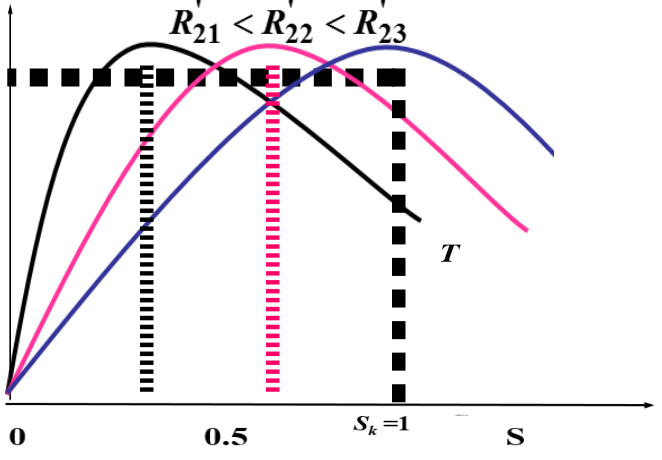
\includegraphics[width=0.6\textwidth,height= 0.6 \textwidth]{yb_rx_jdz.png}
			\caption{转子串入不同电阻\label{figur:yb_rx_jdz}}
		\end{minipage}
		\begin{minipage}[t]{0.48\textwidth}
			\centering
			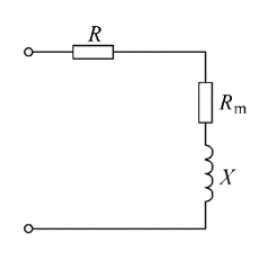
\includegraphics[width=0.6\textwidth,height= 0.6 \textwidth]{pmbzq_dx.png}
			\caption{频敏变阻器等效电路\label{figur:pmbzq_dx}}
		\end{minipage}
	\end{figure}
\end{enumerate}
\subsection{三相异步电动机的软起动}
\begin{enumerate}
	\item (电力电子)常用软起动方式:\\
	定子绕组\underline{串联三对反并联的晶闸管},通过改变晶闸管导通角,调整定子绕组电压,使其按照设定的规律变化。
	\item 优点:
	\begin{itemize}
		\item[-] 灵活控制,起动平稳。
		\item[-] 对电网冲击小,起动损耗小。
		\item[-] 能实现软停车、软制动及断相、过载和欠压等多种保护功能,可实现电动机轻载节能运行。
	\end{itemize}
	\item 缺点:产生谐波,对电网不利。
\end{enumerate}
\section{调速}
$$n=(1-s)n_1=(1-{\color{blue}\boxed{s}})\frac{60{\color{blue}\boxed{f}}}{{\color{blue}\boxed{p}}}$$
\begin{enumerate}
	\item 变转差率$s$调速:
	
	\item 调压调速:{\color{blue}$T_{st}\propto U_{1}^{2}$,$s_k=\frac{r_2^{'}}{x_k}$(不变)}
		\begin{figure}[!hbtp]
			\centering
			\begin{minipage}[t]{0.48\textwidth}
				\centering
				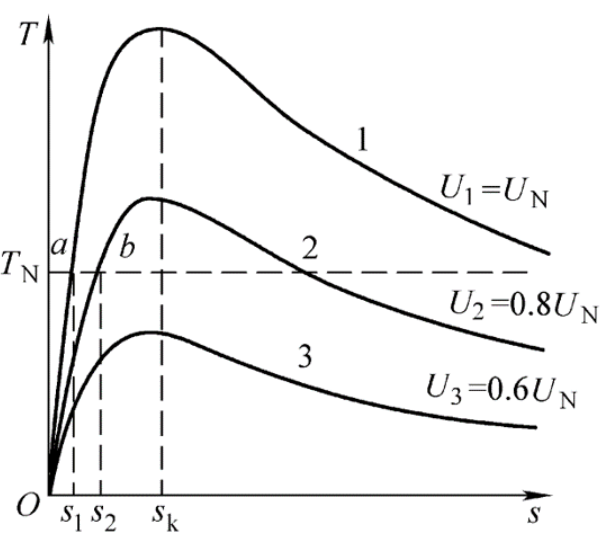
\includegraphics[width=0.6\textwidth,height= 0.6 \textwidth]{dybh_xjtx.png}
				\caption{电压变化的机械特性曲线\label{figur:dybh_xjtx}}
			\end{minipage}
			\begin{minipage}[t]{0.48\textwidth}
				\centering
				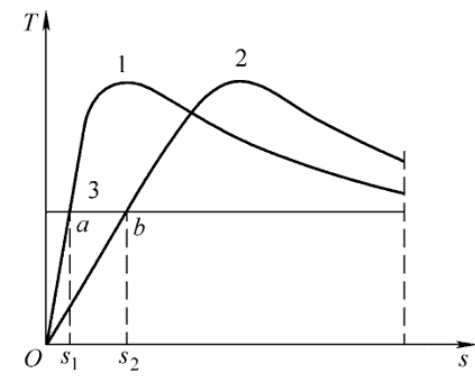
\includegraphics[width=0.6\textwidth,height= 0.6 \textwidth]{czcdz_ts.png}
				\caption{转子串电阻的机械特性曲线\label{figur:czcdz_ts}}
			\end{minipage}
		\end{figure}
		\begin{enumerate}
			\item 转子串电阻调速: 临界转差率$s_k=\frac{r_2^{'}}{x_k}$(变化) $\Rightarrow$机械特性曲线{\color{blue}右移}
			\item 串级调速(双馈调速):在转子回路接一个转差频率的功率变换装置,即{\color{blue}串入频率为$f_2=sf_1$的附加电动势$E_{ad}$},通过{\color{blue}控制$E_{ad}$的大小和相位},将转差功率回馈到电网中去。[节能+调速]
			
			\item 变极调速:改变绕组外部接线or采用两套不同极对数的绕组。
			\begin{figure}[!hbtp]
				\centering
				\subfigure[]{
					\begin{minipage}{0.3\textwidth}
						\centering
						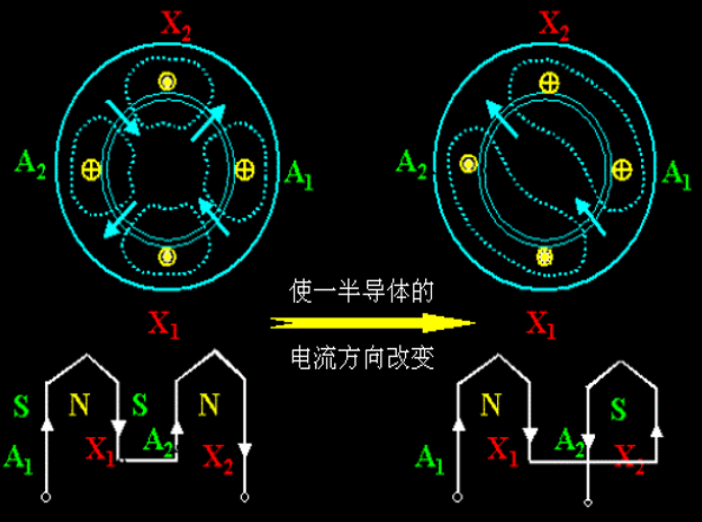
\includegraphics[scale=0.15]{bjts_1.png}
					\end{minipage}
				}
				\subfigure[Y/YY联结改接]{
					\begin{minipage}{0.3\textwidth}
						\centering
						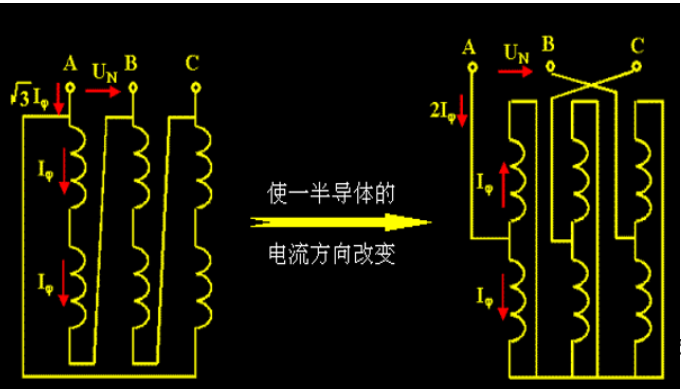
\includegraphics[scale=0.2]{bjts_2.png}
					\end{minipage}
				}
				\subfigure[$\Delta$/YY联结改接]{
					\begin{minipage}{0.3\textwidth}
						\centering
						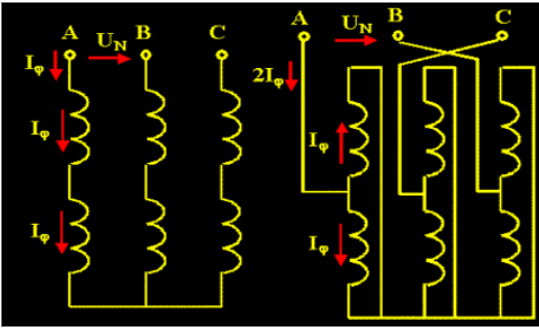
\includegraphics[scale=0.25]{bjts_3.png}
					\end{minipage}
				}
				\caption{变极调速}                    
				\label{figur:bjts}                                                        
			\end{figure}
			\item 变频调速\\
			基频:异步电动机额定频率
			\begin{itemize}
				\item 从基频向下调节:
				\\{\color{thid}降低$f$的同时,也必须降低电源电压$U_1$。}\\
				(1)拖动恒转矩负载时,保持$\Phi_m$不变$\Rightarrow\frac{U_1}{f_1}\approx\frac{E_1}{f_1}$不变\\
				(2)拖动风机负载低速运行时,{\color{blue}为减小铁耗},使$\Phi_m$低于额定值,即$\frac{U_1}{f_1}$比不变时低一些。
				\begin{note}
					从$U_1\approx E_1=4.44f_1N_1\Phi_mk_{w1}$看出,$U_1$不变时,$f$减小,$\Phi_m$增大(正常情况下,主磁路处于饱和点),主磁路过于饱和$\Rightarrow$磁阻增大,励磁电流增大,铁耗增大,功率因数降低。
				\end{note}
				\item 从基频向上调节:通过变频器实现
				\begin{note}
					从$U_1\approx E_1=4.44f_1N_1\Phi_mk_{w1}$看出,$U_1$不变时,$f$增大,$\Phi_m$减小,$T_{max}$减小,不适合驱动恒转矩负载。
				\end{note}
			\end{itemize}
		\end{enumerate}
		\section{制动}
		\begin{enumerate}
			\item 机械制动:由机械方式(如制动闸)施加制动转矩而实现的制动。
			\item 电气制动:施加于电动机的电磁转矩方向与转速方式反向,迫使电动机减速或停止转动。
			\begin{itemize}
				\item 能耗制动:{\color{blue}定子}从交流电源断开,{\color{blue}接直流电源。}
				($n_1>n\Rightarrow n_1=0<n$)
				\begin{note}
					转子具有惯性,继续按原方向转动;定子电流在气隙产生{\color{blue}恒定磁场}。运动的转子切割磁场,产生感应电动势和电流,从而产生{\color{blue}电磁转矩},此转矩与定子由于{\color{blue}惯性}作用而旋转的方向相反,起{\color{blue}制动}作用,迫使定子停下来。
				\end{note}
				\item 回馈制动(再生制动):在{\color{blue}外力}作用下,{\color{blue}转子转速超过同步转速},则电磁转矩和转子转速方向相反,起制动作用。{\color{blue}(发电状态)}
				($n_1>n\Rightarrow n_1<n$)
				\item 反接制动:{\color{blue}改变气隙磁场的旋转方向},使电磁转矩和转子转速方向相反,成为制动转矩。
				\\(1)改变电源相序($n_1\approx n\Rightarrow n_1$反向后,相差$2$倍左右)
				\\优点:制动迅速;
				\\缺点:制动电流大,需要采取限流措施,且能耗大,振动和冲击力也大。
				\\(2)负载转矩使电动机反转{\color{blue}(外力)}
			\end{itemize}
		\end{enumerate}
	\end{enumerate}


\chapter{三相异步电动机的异常运行(12)}
\begin{enumerate}
	\item 非额定电压,非额定电源运行(负载转矩$T_L$不变时):
	\begin{table}[htb]
		\centering
		
		\begin{tabular}{|c|c|c|c|c|c|c|c|c|c|c|c|c|c|}
			\hline 
			& $\Phi_m$ & $x_1$ & $x_2^{'}$ & $I_m$ & $I_1$ & $I_2^{'}$ & $s$ & $n$ & $T$ & $\cos\phi$ & $\eta$ & $p_{Fe}$  & $p_{Cu}$ \\ \hline
			$U_{1}<U_{N}$(轻载) & $\downarrow$ & -- & $\downarrow$ & $\Downarrow$ & $\downarrow$ &  & $\uparrow$ & $\downarrow$ & -- & $\uparrow$ &  $\uparrow$ & $\Downarrow$ & $\uparrow$ \\ \hline
			
			$U_{1}<U_{N}$(重载) & $\downarrow$ & -- & $\downarrow$  & $\downarrow$ & $\uparrow$ & $\Uparrow$  & $\uparrow$ & $\downarrow$ & -- &  $\downarrow$ & $\downarrow$ & $\downarrow$ & $\Uparrow$ \\ \hline
			
			$U_{1}>U_{N}$ & $\uparrow$ & -- & $\uparrow$ & $\Uparrow$  & $\uparrow$ &  & $\downarrow$ & $\uparrow$ & -- & $\downarrow$ & $\downarrow$ & $\uparrow$ &$\downarrow$ \\ \hline
			
			\hline\hline
			
			$f_{1}>f_{N}$ & $\downarrow$ & $\uparrow$ & $\uparrow$ & $\downarrow$ & $\downarrow$ & & $\downarrow$&$\uparrow$   &-- & $\uparrow$  & $\uparrow$ & $\downarrow$ &  \\ \hline
			
			$f_{1}<f_{N}$ & $\uparrow$ & $\downarrow$ & $\downarrow$& $\Uparrow$ & $\uparrow$ & & $\uparrow$ & $\downarrow$ & -- & $\downarrow$ &  $\downarrow$ & $\uparrow$ & $\uparrow$ \\ \hline
			
		\end{tabular}
	\end{table}
	
	\begin{note}
		\begin{itemize}
			\item 励磁电阻$r_m$和励磁电抗$x_m$都随主磁路饱和程度$\Uparrow$而$\Downarrow$
			\item $T=\frac{pm_1}{2\pi f_1}U_1^{2}\frac{\frac{r_2^{'}}{s}}{(\frac{r_2^{'}}{s})^{2}+x_k^{2}}$,$f_1\uparrow$(或$U_1\downarrow$),相同的s对应的$T\downarrow$
		\end{itemize}
	\end{note}
	\item 不对称电源电压和电源缺相时运行,用{\color{thid}对称分量法}分析。
\end{enumerate}

\section{非额定电压下的运行}
实际电压与额定电压之差不能超过{\color{thid}$\pm5\%$}
\begin{note}
	因为${\color{blue}T_{st}\propto U_{1}^{2},I_{st}\propto U_{1}}$,电压降低可能带不动负载,引起电压过热。
\end{note}
\begin{enumerate}
	\item 电源电压$<$额定电压\\
	从$U_1\approx E_1=4.44f_1N_1\Phi_mk_{w1}$可以看出,此时$E_1\downarrow$,$\Phi_m\downarrow$。又因为$T=C_T\Phi_mI_2^{'}\cos\phi_2$,负载转矩不变时,转差率$s\uparrow$,转子电流$\uparrow$。又因为{\color{blue}$P_{Cu2}=sP_{em}=sT\Omega_1$},转子铜耗$\uparrow$。
	\begin{itemize}
		\item {\color{blue}轻载时,转子电流和转子铜耗}{\color{blue}较小,在定子电流$I_1$的励磁分量$I_m$和负载分量$I_L$中,$I_m$起主要作用}($s$小,等效电路中$\frac{r_2^{'}}{s}\approx \infty $,转子侧相当于开路)。当$U_1\Downarrow$时,$I_m\Downarrow$,定子电流$I_1\Downarrow$,{\color{thid}定子功率因数$\cos\phi_1\uparrow$}。同时,轻载时,$p_{Fe}\gg p_{Cu}$,当$U_1\Downarrow$时,$\Phi_m\Downarrow$,$p_{Fe}\Downarrow$,{\color{thid}$\eta \Uparrow$}。\\
		电动机轻载时,端电压降低对电机运行有利。实际中,可将正常运行时三角形联结的定子绕组,在轻载时改成星型联结。
		\begin{note}
			{\color{main2}转子功率因数$\cos\phi_2\Downarrow$怎么变?}
		\end{note}
		\item {\color{blue}重载时,转子电流较大,在定子电流$I_1$的励磁分量$I_m$和负载分量$I_L$中,$I_L$起主要作用}($s$大,等效电路中$\frac{r_2^{'}}{s} $较小,转子电流较大)。当$U_1\Downarrow$时,$s\Uparrow$,$I_2\Uparrow$,定子电流$I_1\Uparrow$,{\color{thid}转子功率因数$\cos\phi_2\Downarrow$,定子功率因数$\cos\phi_1\Downarrow$($s\Uparrow$)}。同时,重载时,当$U_1\Downarrow$,$\Phi_m\Downarrow$,$p_{Fe}\downarrow$,但$p_{Cu}$随电流二次方增加而$\Uparrow$,{\color{thid}$\eta \Downarrow$}。
		\begin{note}
			{\color{main2}为什么转差率$\Uparrow$,转子功率因数$\cos\phi_2\Downarrow$,定子功率因数$\cos\phi_1\Downarrow$?}
		\end{note}
	\end{itemize}
	\item 电源电压$>$额定电压\\
	当$U_1\uparrow$,$\Phi_m\uparrow$,磁路饱和程度大大增加,$I_0\Uparrow$,功率因数$\downarrow$,$p_{Fe}\uparrow$,$\eta \downarrow$
\end{enumerate}
\section{非额定频率下的运行}
实际频率与额定频率之差不能超过{\color{thid}$\pm1\%$}。{\color{blue}在不考虑定子绕组漏阻抗压降时},$U_1\approx E_1=4.44f_1N_1\Phi_mk_{w1}$,保持电源电压$U_1$不变时,$\Phi_m\propto 1/f_1$。
\begin{enumerate}
	\item 电网频率>额定频率时,$\Phi_m\downarrow$,励磁电流$I_m \downarrow$,\underline{与此同时,定子电流$I_1\downarrow$,转速$n\uparrow$},电动机功率因数、效率和通风冷却等都有所改善。
	\begin{note}
		{\color{main1}划线处是为什么?}
	\end{note}
	\item 电网频率<额定频率时,$\Phi_m\uparrow$,励磁电流$I_m \Uparrow$,定子电流$I_1\uparrow$,$p_{Fe}\uparrow$,$p_{Cu}\uparrow$,\underline{功率因数$\downarrow$,效率$\eta\downarrow$;同时,电机转速$n\downarrow$,使电机通风冷却条件变差,温升提高。}此时,电动机必须减小负载,使电动机在轻载下运行,防止电动机过热。所以,异步电动机不能在低频下带额定负载运行。当其利用变频调速时,在降低频率调速的同时,要降低电源电压,以保持主磁通恒定。
	\begin{note}
		{\color{main1}划线处是为什么?}
	\end{note}
\end{enumerate}
\section{不对称电源电压下的运行}
采用{\color{thid}对称分量法},把不对称的三相电压分解为正序,负序和零序分量。又因为异步电动机定子绕组一般为星型无中心线或三角形联结,{\color{thid}所以没有零序电压,零序电流和零序磁通}。因为负序磁场反转,所以负序电流的转差率为$$s_{-}=\frac{-n_1-n}{-n_1}=\frac{2n_1}{n_1}-\frac{n_1-n}{n_1}=2-s$$
$2-s>1$,$s<1$,负序等效电路中,转子等效电阻更小,负序电流会较大。\\负序电流$\rightarrow$负序磁动势$\rightarrow$负序感应电流$\rightarrow$负序电磁转矩$T_{-}$(与转子转动方向相反,起制动作用)。\\
负序分量影响:由于负序转矩的出现,电机合成转矩减小,导致电动机启动转矩和过载能力下降。负序磁场以2倍同步转速切割转子绕组,转子铁耗$\Uparrow$,$\eta\downarrow$,转子温度升高。
\section{电源缺相时的运行}
对称分量法

\chapter{三相同步发电机的基本工作原理与结构(14)}
同步发电机的特点:
\begin{itemize}
	\item  转子转速$n$=旋转磁场转速$n_1$
	$$n=n_1=\frac{60f}{p}$$
	设计好的同步发电机,只要电源频率不变,转速恒定。
	\item  {\color{thid}双边励磁},转子绕组需要通入直流电流,产生机械旋转磁场。
\end{itemize}
\section{同步发电机的基本工作原理及分类}	
\begin{enumerate}
	\item 基本原理:{\color{blue}定子(电枢)}铁心上的励磁绕组,通有直流电流,产生励磁磁场。原动机拖动电枢旋转,励磁磁场随之旋转,形成机械旋转磁场,该磁场依次切割定子各相绕组,产生交流电动势。如果接上负载,就有电流流过,此时发电机将有电流流过,实现机械能转化为交流电能。
	\item 分类:
	\begin{itemize}
		\item 按运行方式分:发动机,电动机和调相机。
		\item 按结构形式分:电枢旋转式(转枢式),磁极旋转式(转场式)。
		\item 按转子结构分:凸极式,隐极式。
		\item 按安装方式:卧式,立式。
		\item 按原动机类型:汽轮发电机,水轮发电机,etc.
		\item 按冷却介质分:空气冷却,氢气冷却,水冷却,etc.
	\end{itemize}
\end{enumerate}
\section{同步发电机的基本结构}
\begin{itemize}
	\item 凸极式适用于低转速(极对数$p$较多),e.g.汽轮发电机
	\item 隐极式适用于高转速(极对数$p$较少),e.g.水轮发电机
	\item \underline{同步电机气隙要比容量相同的异步电机大。}异步电机的励磁电流由电网供给,需要从电网吸收感性无功电流来励磁(如果气隙大,则励磁电流大,电机的功率因数低,因此,在机械允许的条件下,气隙要尽量小一点)
	\item 对于同步电动机,气隙大,同步电抗小,短路比【系统短路容量/设备容量。短路比大,表明设备的投切对系统影响不是很大】大,运行稳定性高。{\color{thid}但是},气隙大,转子用铜量增大,制造成本增加。
\end{itemize}
\subsection{汽轮发电机}
\begin{enumerate}
	\item 定子=机座+端盖+定子铁心+定子绕组,etc
	\item 转子(隐极式,细而长)=转子铁心+励磁绕组+阻尼绕组+紧固件(护环和中心环)+风扇,etc
	\item 冷却系统
	\item 集电环和电刷等其他部件
\end{enumerate}
\subsection{水轮发电机}
\begin{enumerate}
	\item 定子=机座+定子铁心+定子绕组,etc
	\item 转子(凸极式,大而短)=转轴+转子铁心+励磁绕组+转子支架+磁轭+磁极,etc.磁极固定在磁轭上,磁轭同时也是磁路的组成部分。
	\item 冷却系统
	\item 集电环和电刷等其他部件
\end{enumerate}
\section{大型同步发电机的基本系统}
\subsection{同步发电机的绝缘与冷却}
\begin{enumerate}
	\item 绝缘系统:主要是定子绕组和转子绕组绝缘。
	\begin{itemize}
		\item 定子绕组绝缘:匝间,层间,对地(槽绝缘)及连接线和引出线的绝缘。
		\item 转子绕组绝缘:匝间,对地和引出线绝缘。
	\end{itemize}
	\item 温升要求
	\item 冷却系统:\\
	300MW水氢氢系统:(书P210-P211)	
\end{enumerate}
\subsection{同步发电机的励磁}
\begin{enumerate}
	\item 要求:随负载情况变化,励磁电流能相应调节(系统电压严重下降时,能强行励磁,提高电动势;突然甩负荷时,能强行减磁,限制端电压过度增高)。
	\item 励磁方式:
	\begin{itemize}
		\item 直流励磁机励磁:\\与同步发电机转子同轴的直流发电机作为励磁电源。(并励,他励,负载电流反馈的复式励磁接法)
		\item 静止整流器励磁:\\(主发电机+交流主励磁机+交流副励磁机)\\副励磁机的励磁电流开始由外部直流电源提供,电压建立起来后,转为自励(有时采用永磁发电机)。副励磁机及输出电流经(静止晶闸管整流器)整流后供给主励磁机,而主励磁机的输出电流经(静止的三相桥式二极管整流器)整流后,通过{\color{blue}电刷和集电环}供给主发电机的励磁绕组。
		\item 旋转整流器励磁:\\(主发电机+交流主励磁机{\color{blue}(旋转电枢式三相同步发电机,二极管整流器一起旋转)}+交流副励磁机)\\
	\end{itemize}
\end{enumerate}
\section{同步电机的型号与额定值}
\begin{enumerate}
	\item 型号:
	\begin{itemize}
		\item QF(汽轮发电机)/TS(水轮发电机)+Q(氢外冷)/N(氢内冷)/S(双水内冷)
		\item TD(同步电动机)+G(高速)/L(立式)
		\item TT(同步调相机)\newpage
		\item QFS-300{\color{thid}-2}:容量为300MW双水内冷{\color{thid}2极}汽轮发电机
		\item TSS1264/160{\color{thid}-48}:双水内冷水轮发电机,定子外径1264cm,铁心长160cm,{\color{thid}极数48}
		\item TS854-210-40:
	\end{itemize}
	\item 额定值: {\color{blue}除了额定容量是有功功率(kW)},其它和异步电机的描述差不多。
\end{enumerate}

\chapter{三相同步发电机的运行原理(15)}
\section{同步发电机的空载运行}
\subsection{空载运行时的电磁过程}
\begin{figure}[!hbtp]
	\centering
	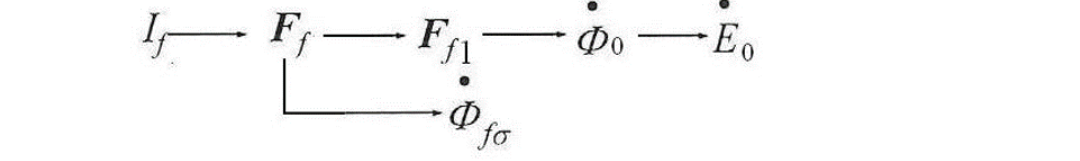
\includegraphics[width=0.9\textwidth,height= 0.15 \textwidth]{tb_kz.png}
	\caption{空载运行时的电磁过程\label{figur:tb_kz}}
\end{figure}
{\color{thid}因为主磁通$\Phi_0$和转子转速相同,只在定子感应电动势和漏磁通,在转子侧没有感应电动势。}建立空载磁场的励磁磁动势$F_f$的 大小与空间分布和电机结构有关。\\
\begin{enumerate}
	\item 隐极式发电机
	\begin{itemize}
		\item 其励磁绕组嵌埋于转子槽内,沿转子圆周气隙可视为均匀。
		\item 励磁磁动势$F_f$在空间分布为{\color{thid}阶梯形},用谐波分析法可以求出其空间基波分量$F_{f1}$(书P216)
	\end{itemize}
	\item 凸极式发电机
	\begin{itemize}
		\item 其励磁绕组集中放置在转子磁极上,沿转子圆周气隙不均匀,极面下气隙较小,磁阻较小,而极间气隙大,磁阻较大,因而$F_{f1}$建立的气隙磁场在一个极的范围内,气隙径向磁通密度的分布近似于平顶的帽形,极靴以外的气隙磁通密度减小很快。
		\item 励磁磁动势$F_f$在空间分布为{\color{thid}矩形},用谐波分析法可以求出其空间基波分量$F_{f1}$(书P216)
	\end{itemize}
\end{enumerate}
\subsection{空载特性}
\begin{enumerate}
	\item 空载特性$E_)=f(I_f)$或$E_0=f(F_f)$:
	空载特性与电机磁路的磁化曲线具有类似的变化规律。
	\begin{itemize}
		\item 励磁电流较小时,由于磁通较小,磁路没有饱和,空载特性呈直线。
		\item 随着励磁电流增大,磁路逐渐饱和,空载电动势增加一点,励磁磁动势增加很多。
		\item 为了合理利用材料,又不因过分饱和增加励磁磁动势而增加用铜量,空载额定电压一般选在空载特性的刚好弯曲处(c点)。
		\item 饱和系数:$$k_s=\frac{\overline{ac}}{\overline{ab}}=\frac{\overline{dn}}{\overline{Oa}}=\frac{E^{'}_0}{U_N}$$
		磁路饱和后,由励磁磁动势建立的基波主磁通和感应的基波电动势都降为未饱和值的$\frac{1}{k_s}$,或者说所需磁动势是未饱和时的$k_s$倍(即$F_f=k_sF_{\sigma}$)
	\end{itemize}
	\begin{note}
		根据空载时的电磁过程,每相定子绕组的基波感应电动势大小为$E_0=4.44fN\Phi_0k_{w1}\Rightarrow E_0\propto\Phi_0$,又因为$F_f=NI_f\Rightarrow F_f\propto I_f$,$F_f=Hl\Rightarrow F_f\propto H$,$\Phi_0=BS\Rightarrow \Phi_0\propto B$,所以,空载特性曲线和电机磁路的磁化曲线具有类似变化规律。
	\end{note}	
	\begin{figure}[!hbtp]
		\centering
		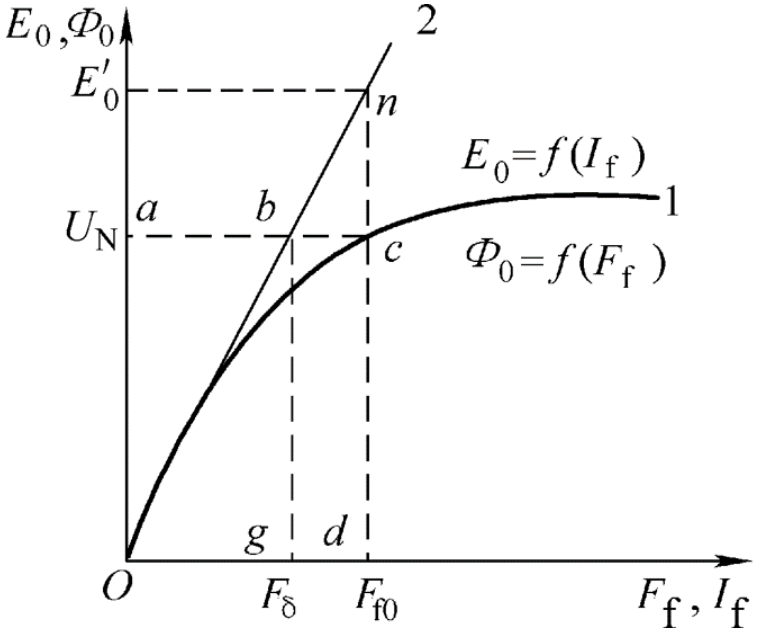
\includegraphics[width=0.5\textwidth,height= 0.35 \textwidth]{tb_kz_dc.png}
		\caption{1—空载特性曲线\quad2—气隙线\label{figur:tb_kz_dc}}
	\end{figure}
	\item 空载运行时空相矢图:\\
	同步发电机的励磁磁动势(空间矢量)是以同步转速$\Omega_1$在空间旋转,定子绕组感应产生的频率$\Omega_1$的正弦基波电动势(时间相量)在时间上呈同步变化。
	\begin{itemize}
		\item 直轴(纵轴/d轴):主磁极轴线位置。
		\item 交轴(横轴/q轴):磁极N、S之间的中心线,与d轴成90度{\color{thid}电角度}
		\item 相轴:相绕组轴线位置
		\item 时轴:时间相量在其上投影可得瞬时值
	\end{itemize}
	\begin{figure}[!htp]
		\centering
		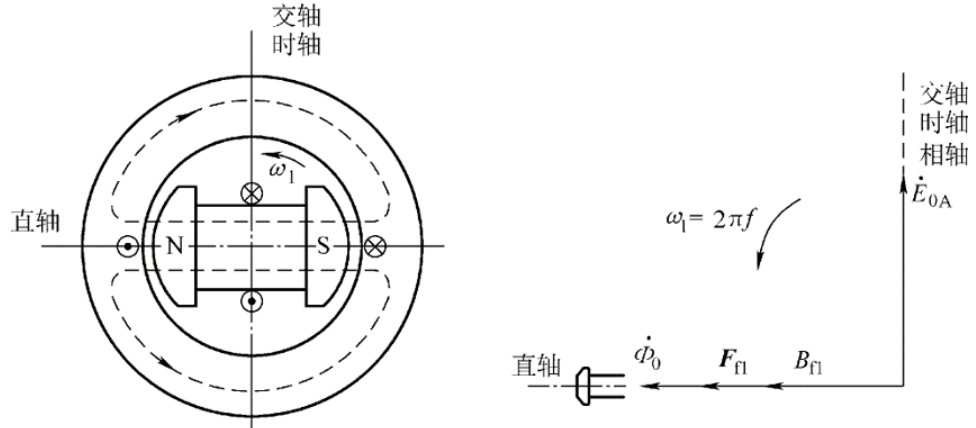
\includegraphics[scale=0.5]{kzyx_skxs.png}
		\caption{空载运行时空相矢图}
	\end{figure}
	\item 电压波形正弦性的畸变率:
	$$K_u=\frac{100}{u_1}\sqrt{u_2^{2}+u_3^{2}+\ldots+u_n^{2}}$$
	$u_1$—基波电压有效值,也可用线电压的有效值代替;$u_n$—$n$次谐波电压有效值。
\end{enumerate}
\subsection{同步发电机带对称负载}
\begin{enumerate}
	\item {\color{thid}没有磁动势平衡}:\\
	转子电流只有励磁分量,没有负载分量。
	\begin{note}
		与变压器和异步电动机不一样的是,同步发电机是双边励磁。同步发电机的转子侧,通入的是直流电流,产生的是恒定不变的励磁磁动势,随转子转动形成机械旋转磁动势$F_f$。而且,由于这个机械旋转磁动势和转子转速相等,转子侧不会产生感应电动势(转子不切割主磁通和转子侧漏磁通);而定子侧切割主磁通和定子侧漏磁通,产生感应电流,继而产生与$F_f$同步的电枢磁动势。	
	\end{note}	
	\item 电枢反应:电枢磁动势的出现,使气隙磁场的大小和位置发生改变。所有的电枢反应都可以分解为:去磁电枢反应,助磁电枢反应,交磁电枢反应,可以用时空相矢图来分析。
	\begin{note}	
		因为励磁磁动势和电枢磁动势同步,相对静止,所以可以选取任一时刻分析(把时轴放到需要的地方),结果一样。定义以下角度:
		\begin{itemize}
			\item $\psi$:励磁磁动势$\dot{E_0}$和电枢电流$\dot{I_a}$之间的相位差
			\item 外功率因数角$\upvarphi$:电枢输出电压$\dot{U}$和$\dot{I_a}$之间的相位差
			\item 功(率)角$\delta$:定子绕组感应电动势$\dot{E_0}$和$\dot{U}$之间相位差
		\end{itemize}
	\end{note}
	\begin{table}[!htbp]
		\centering
		\caption{三种基本的电枢反应}
		\begin{tabular}{|c|c|c|c|c|c|c|c|}
			\hline
			电枢磁动势方向 & 作用    & $\Psi$ & 转矩 & 气隙磁场  & 端电压   & 调节方法  & 负载性质 \\\hline
			交轴    & 交磁    & $0$\textdegree & 制动    & 增强 & 不变    & 输入更多机械功率 & 纯电阻 \\\hline
			直轴    & 去磁    & $90$\textdegree & 无     & 不变    & 降低    & 增大励磁电流 & 纯电感 \\\hline
			直轴    & 增磁    & $-90$\textdegree & 无     & 不变    & 增大    & 减小励磁电流 & 纯电容 \\\hline
		\end{tabular}%
		\label{tab:addlabel1}%
	\end{table}%
	\begin{figure}[!hbtp]
		\centering
		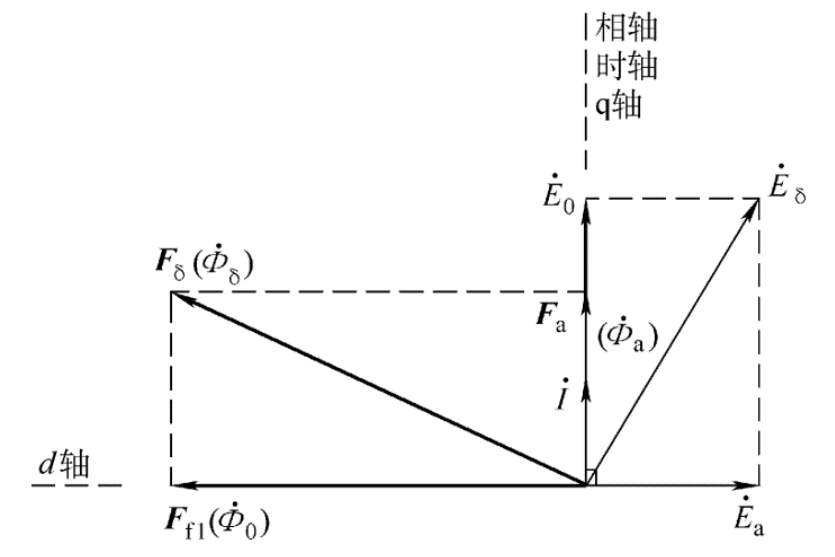
\includegraphics[scale=0.35]{sk_ds_1.png}
		\caption{$\Psi=0 \degree$时的时空相矢图}                 
		\label{figur:sk_ds_1}                                   
	\end{figure}
	\begin{figure}[!hbtp]
		\centering
		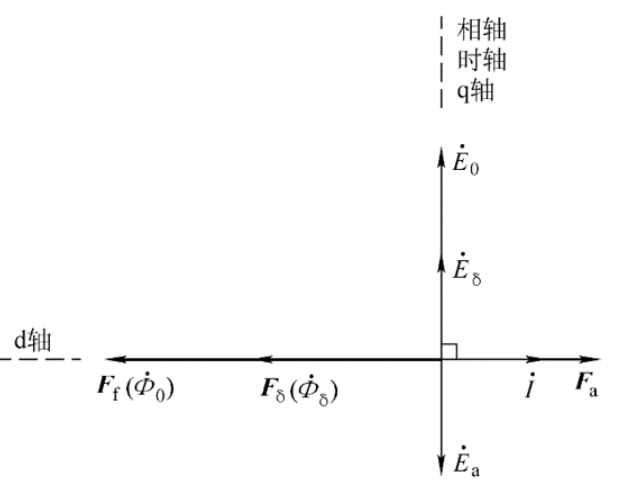
\includegraphics[scale=0.35]{sk_ds_2.png}
		\caption{$\Psi=90 \degree$时的时空相矢图}                 
		\label{figur:sk_ds_2}                                   
	\end{figure}	
	\begin{figure}[!hbtp]
		\centering
		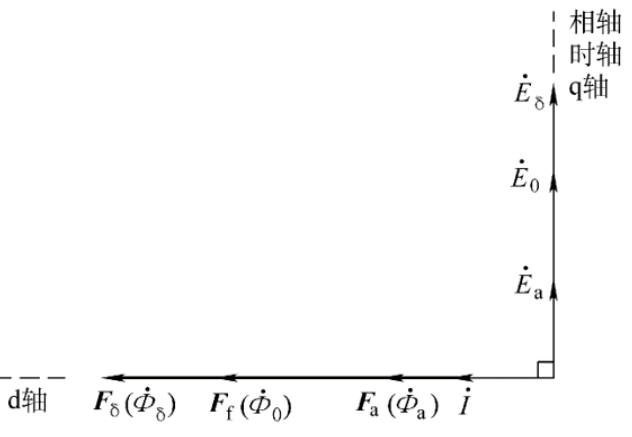
\includegraphics[scale=0.35]{sk_ds_3.png}
		\caption{$\Psi=-90 \degree$时的时空相矢图}                 
		\label{figur:sk_ds_3}                                   
	\end{figure}
\end{enumerate}
\subsection{隐极同步发电机的负载运行}
\begin{enumerate}
	\item 磁路不饱和时:
	\begin{itemize}
		\item 电磁关系:
		\begin{figure}[!hbtp]
			\centering
			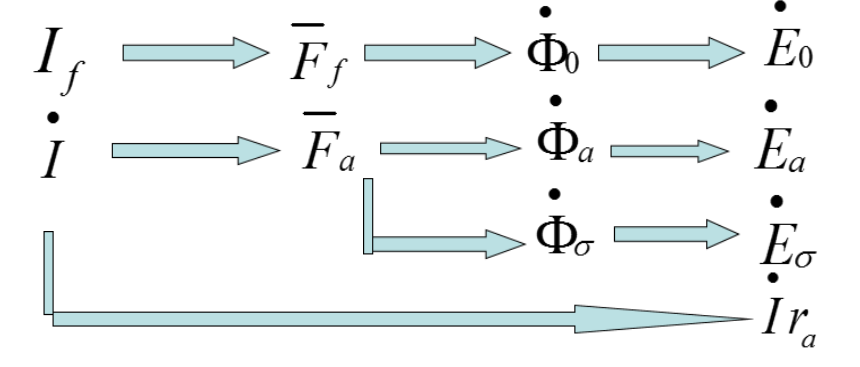
\includegraphics[scale=0.25]{yj_bhh_dcgx.png}
			\caption{磁路不饱和时隐极同步发电机电磁关系}           \label{figur:yj_bhh_dcgx}                           
		\end{figure}
		\begin{figure}[!hbtp]
			\centering
			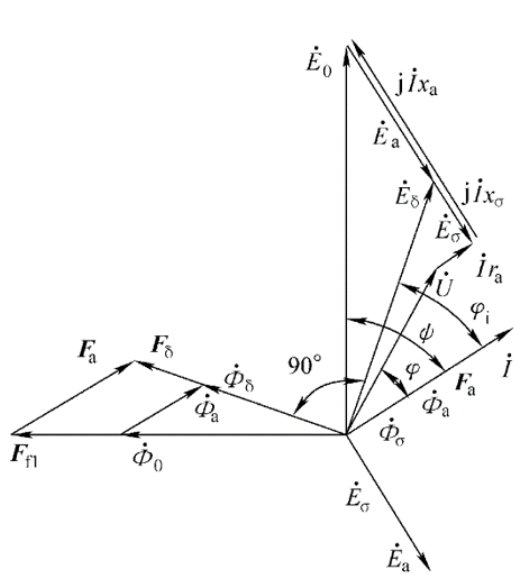
\includegraphics[scale=0.4]{yj_bhh_skxs.png}
			\caption{磁路不饱和时隐极同步发电机时空相矢图}           \label{figur:yj_bhh_skxs}                           
		\end{figure}
		\item 等效电路和向量图:
		\begin{align*}
		\dot{E_0}&=\dot{U}+\dot{I}r_a+j\dot{I}x_a+j\dot{I}x_{\sigma}\\&=\dot{U}+\dot{I}r_a+j\dot{I}x_s\\&=\dot{U}+\dot{I}Z_s
		\end{align*}
		其中$x_s$为同步电抗,$x_a$为电枢反应电抗,$x_{\sigma}$为定子漏电抗,有$x_s=x_a+x_{\sigma}$;$Z_s$为同步阻抗,$Z_s=r_a+x_s$,所以等效电路和向量图如下。
		\begin{figure}[!hbtp]
			\centering
			\subfigure[向量图]{
				\begin{minipage}{0.3\textwidth}
					\centering
					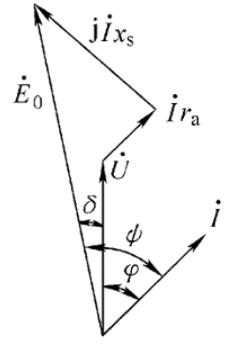
\includegraphics[scale=0.4]{yj_bhh_xlt.png}
				\end{minipage}
			}
			\subfigure[等效电路1]{
				\begin{minipage}{0.45\textwidth}
					\centering
					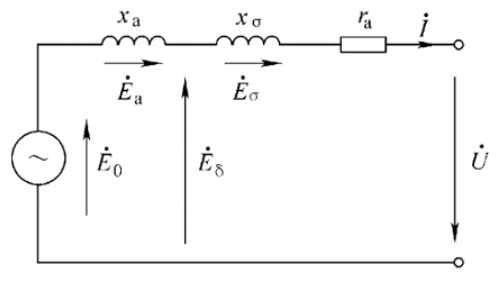
\includegraphics[scale=0.4]{yj_bhh_dxdl1.png}
				\end{minipage}
			}
			\subfigure[等效电路2]{
				\begin{minipage}{0.3\textwidth}
					\centering
					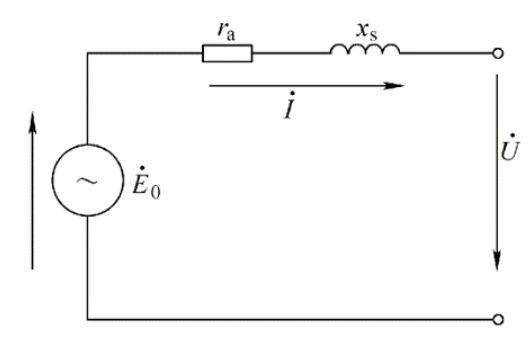
\includegraphics[scale=0.4]{yj_bhh_dxdl2.png}
				\end{minipage}
			}
			\caption{磁路不饱和时隐极同步发电机等效电路和向量图}      
		\end{figure}
	\end{itemize}
	\item 磁路不饱和时:电磁关系和不饱和时一样,但是{\color{thid}叠加定理不再适用,即$F{\delta}$作用的结果并非$F_a$和$F_{f1}$分别作用效果之和}
	\begin{note}
		$\Phi_0+\Phi_a$不再对应$F_0+F_a$l了,对应的磁动势更大,需要查空载曲线得知。
	\end{note}	
\end{enumerate}
\subsection{凸极同步发电机的负载运行}
\begin{enumerate}
	\item 磁路不饱和时:\\
	由于凸极同步发电机的气隙不均匀,在极面下的磁导大,两极之间的磁导小,同一电枢磁动势波作用在气隙不同处,会遇到不同的磁阻,产生不同的磁通和磁密。为便于计算,引入双反应理论,把电枢基波磁动势$F_a$分解为直轴上的直轴电枢反应 磁动势分量$F_{ad}$和交轴上的交轴电枢反应磁动势分量$F_{aq}$。$F_a$处于不同位置,产生的电枢磁场不同:
	\begin{itemize}
		\item 电枢磁动势作用于$d$轴时,极弧下的气隙磁场$B_{ad}$接近正弦波形。
		\item 电枢磁动势作用于$q$轴时,极弧下的气隙磁场$B_{aq}$接近马鞍波形。 
	\end{itemize} 
	\begin{figure}[!hbtp]
		\centering
		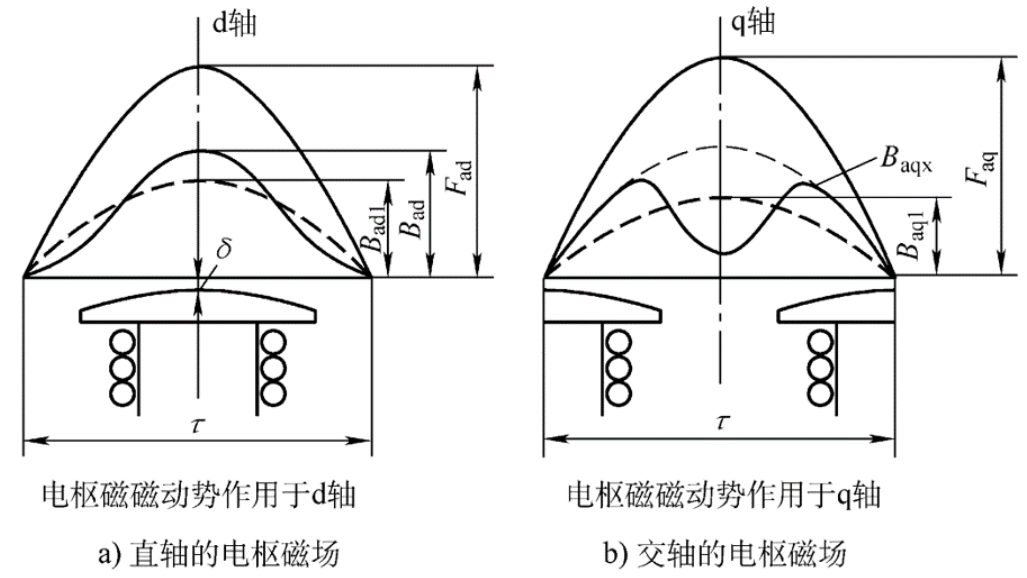
\includegraphics[scale=0.3]{tjtb_bbh_czxz.png}
		\caption{磁路不饱和时凸极同步发电机电磁关系}           \label{figur:tjtb_bbh_czxz}                           
	\end{figure}
	向量图:	
	\begin{align*}
	\dot{E_0}&=\dot{U}+\dot{I}r_a+j\dot{I_d}x_d+j\dot{I_q}x_q\\
	&=\dot{U}+\dot{I}r_a+j\dot{I_d}(x_{ad}+x_{\sigma})+j\dot{I_q}(x_{aq}+x_{\sigma})\\&=\dot{U}+\dot{I}r_a+j\dot{I_d}x_{ad}+j\dot{I_q}x_{aq}+j\dot{I}x_{\sigma}\\\\
	\dot{E_0}&=\dot{U}+\dot{I}r_a+j\dot{I_d}x_d+j\dot{I_q}x_q\\
	&=\dot{U}+\dot{I}r_a+j\dot{I_d}x_d+j\dot{I_q}x_q{\color{blue}\boxed{-j\dot{I_d}x_q+j\dot{I_d}x_q}}\\
	&=\dot{U}+\dot{I}r_a+j\dot{I_d}(x_d-x_q)+j(\dot{I_d}+\dot{I_q})x_q\\
	&=\dot{U}+\dot{I}r_a+j\dot{I_d}(x_d-x_q)+j\dot{I}x_q\\
	\Rightarrow {\color{thid}\dot{E_0}+j\dot{I_d}(x_d-x_q)}&= \dot{U}+\dot{I}r_a+j\dot{I}x_q=\dot{U}+\dot{I}(r_a+jx_q)
	\end{align*}
	其中,$x_{ad}$—直轴电枢反应电抗,$x_{aq}$—交轴电枢反应电抗,它们分别反映出直轴和交轴电枢反应磁通的强弱(由于直轴磁路的磁导比交轴磁路的磁导要大得多,所以$x_{ad}>x_{aq}$)。直轴同步电抗$x_d=x_{ad}+x_{\sigma}$,交轴同步电抗$x_q=x_{aq}+x_{\sigma}$
	\begin{itemize}
		\item 确定$q$轴位置\\
		法(1):左边的是一个处于$q$轴位置的相量,先画出右边,然后就可以确定$q$轴的位置。\\
		法(2):$$\Psi=\arctan\frac{U\sin\varphi+x_qI}{U\cos\varphi+Ir_a}$$
	\end{itemize}   
	\begin{figure}[!hbtp]
		\centering
		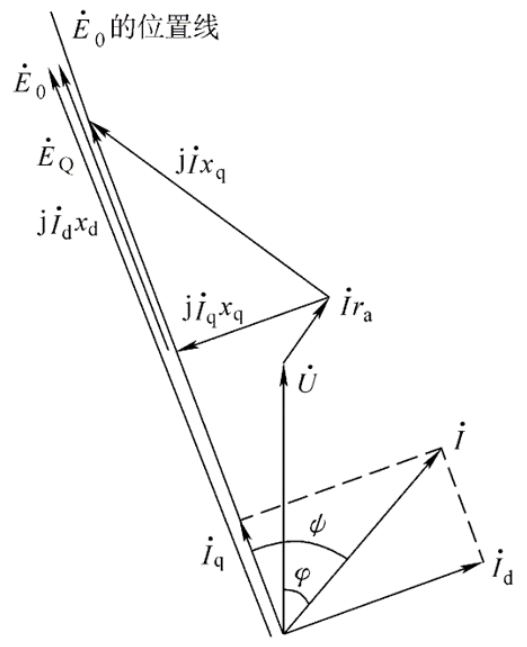
\includegraphics[scale=0.3]{tj_fz_bbh_xl.png}
		\caption{磁路不饱和时凸极同步发电机相量图}           \label{figur:tj_fz_bbh_xl}                           
	\end{figure}
	\item 磁路饱和时:
	\begin{center}
		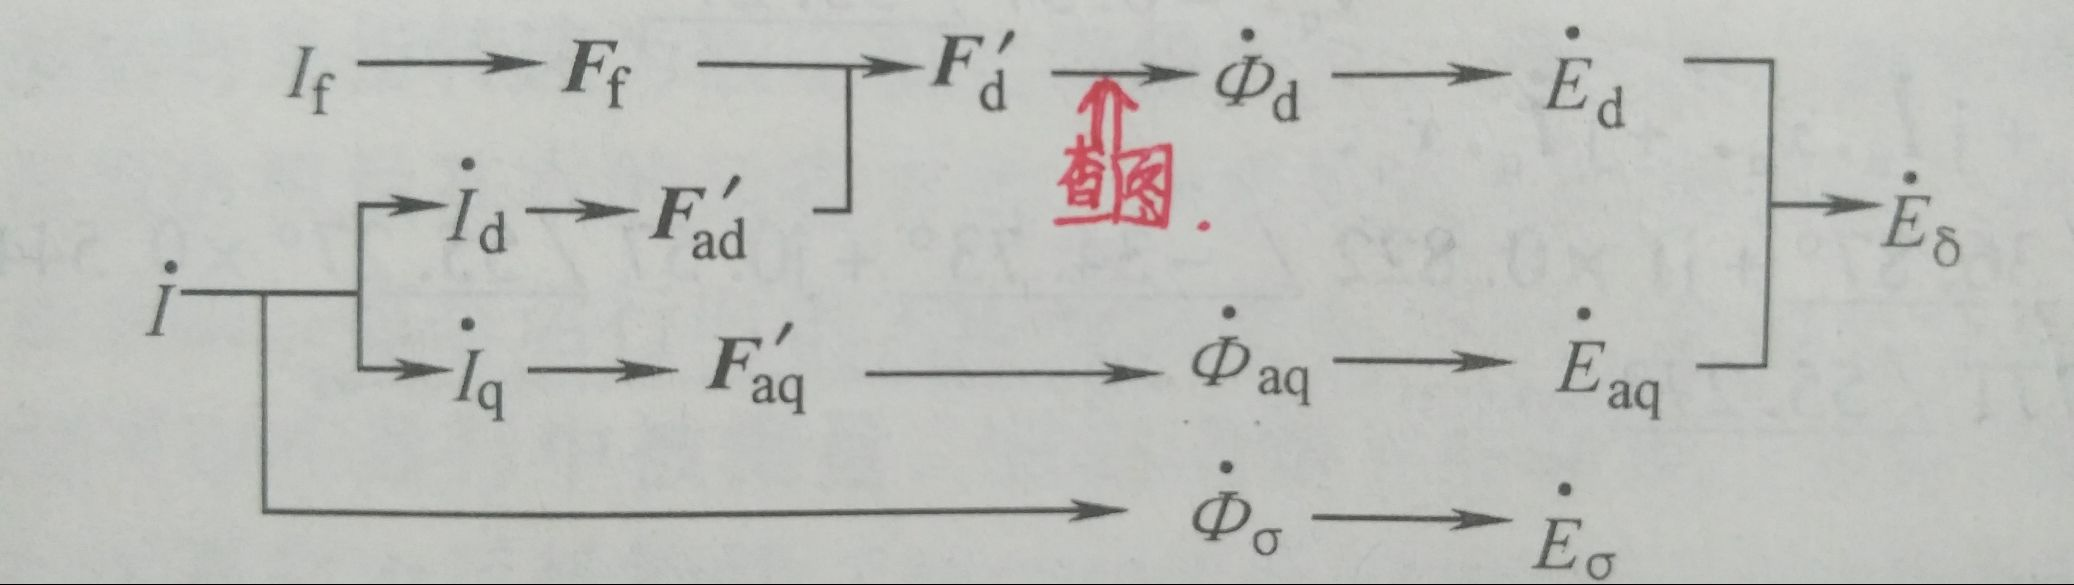
\includegraphics[scale=0.2]{tj_fz_bh.jpg}                  
	\end{center}
\end{enumerate}

\chapter{同步发电机的稳态运行特性及参数的测定(16)}
\begin{enumerate}
	\item 同步发电机稳态运行:{\color{main}转速为额定值且恒定},并供给{\color{main}三相对称负载}时的一种稳态运行方式。
	\item 运行特性:电压$U$,电枢电流$I$,励磁电流$I_f$和功率因数$\cos\varphi$(加上转速一共5个量)中,其它量不变时,两个量之间的关系。
	\item 表征同步发电机运行特性的主要参数为隐极同步电抗$x_s$,凸极同步电抗$x_d$、$x_q$,以及漏抗$x_{\sigma}$等。变量和参数一般采用{\color{blue}标幺值}。由于转子侧是独立回路,基值选取与定子侧无关。{\color{thid}转子电流基值常选空载电动势为额定相电压时的励磁电流值。}
\end{enumerate}

\section{空载特性、短路特性、不饱和同步电抗和短路比的求取}
\subsection{空载特性——$U=f(I_f)$}
由于磁滞现象,上升和下降的曲线不会重合,因此,一般规定采用下降曲线来表示空载特性,再讲将曲线右移,移到过原点处。
\begin{center}
	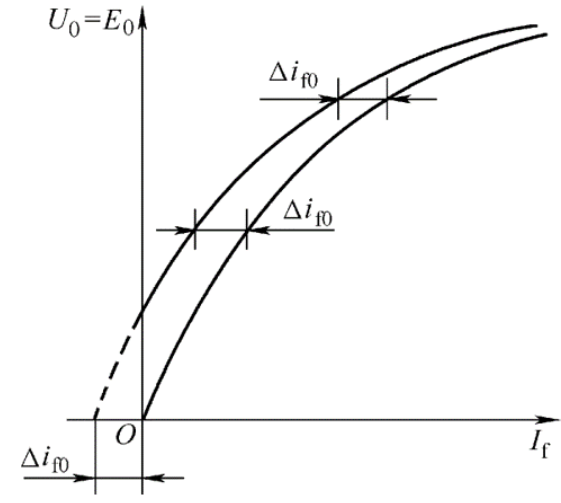
\includegraphics[scale=0.3]{tbfdj_wt_kz.png}                   
\end{center}
\subsection{短路特性——短路电流$I_k=f(I_f)$}
\begin{enumerate}
	\item 
	三相稳态短路($U=0$)\\
	短路特性为一条直线:
	\begin{itemize}
		\item 短路时,限制短路电流的只有发电机的同步阻抗,忽略电枢电阻,只考虑同步电抗,短路电流可看做纯感性。于是$\dot{I_q}=0$,$\dot{I_k}=\dot{I_d}$,此时,电枢反应为去磁作用,因此气隙合成磁动势$F_{\delta}=F_{f1}-F_{ad}$,产生气隙感应电动势$\dot{E_{\delta}}=\dot{U}+\dot{I}r_a+j\dot{I}x_{\sigma}\approx j\dot{I}x_{\sigma}$。
		\item 由于$\dot{E_{\delta}}$只与漏抗压降平衡,数值不大,对应的气隙合成磁通和气隙合成磁动势就很小,磁路处于不饱和状态,则$E_0 \propto I_f$。
		\item 又由于 $\dot{E_{0}}=\dot{U}+\dot{I}r_a+j\dot{I_d}x_d+j\dot{I_q}x_q\approx j\dot{I_k}x_{d}$,则{\color{blue}$I_k \propto E_0$}
		\item 所以{\color{blue}$I_k \propto I_f$}(直线)
	\end{itemize}
	\begin{figure}[!hbtp]
		\centering
		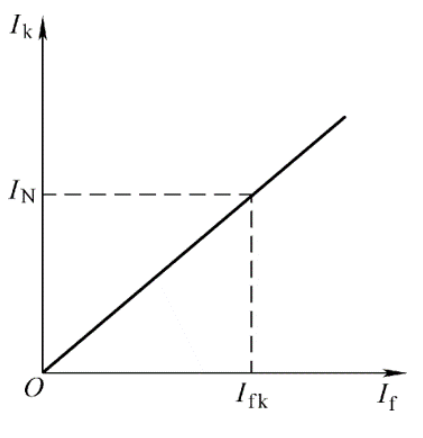
\includegraphics[scale=0.3]{Screenshot_2018-10-28-21-27-34-0782274930.png}
		\caption{短路特性}                         
	\end{figure}
	\item	短路比:【相似三角形得到】({\color{thid}$I_{fk}$:短路时使短路电流为额定值的励磁电流})
	$$k_c=\left.\frac{I_k}{I_N}\right|_{I_f=I_{f0}}=\frac{I_{f0}}{I_{fk}}$$	
		\begin{center}  
		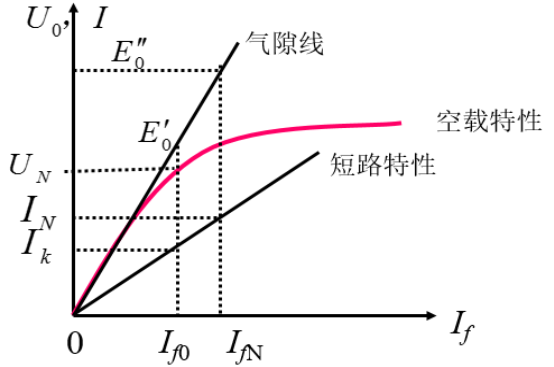
\includegraphics[scale=0.4]{Screenshot_2018-10-28-21-50-44-1949642786.png}
		\captionof{figure}{利用短路特性与短路特性}                     
	\end{center}  
	\item	直轴同步电抗{\color{thid}$x_d$不饱和值}的求取:\\
	\begin{itemize}
		\item 选取一固定$I_f$(如{\color{thid}$I_{f0}$:空载电动势=额定电压时的励磁电流}),求得短路电流$I_k$对应气隙线上的电动势$E_0^{'}$,则:
		$$x_{d{\text {(不饱和值)}}}=\frac{E_0^{'}}{I_k}$$
		标幺值求法1:
		$$x_{d{\text {(不饱和值)}}}^{*}=\frac{x_d}{z_b}=\frac{E_0^{'}}{I_k} \frac{I_{N\phi}}{U_{N\phi}}=\frac{E_0^{'*}}{I_k^{*}} $$
		\item 标幺值求法2:\\
			$$x_{d{\text {(不饱和值)}}}^{*}=\frac{x_{d{\text {(不饱和值)}}}}{z_b}=\frac{E_0^{'}}{I_k}\left/ \frac{U_{N\phi}}{I_{N\phi}}\right.=\frac{E_0}{U_{N\phi}}\frac{I_N}{I_k}=k_s\frac{1}{k_c} $$
			即,
			$$k_ck_{d\text{(不饱和值)}}^{*}=k_s$$
			\begin{note}
				短路比$k_c$的影响:
				\begin{itemize}
					\item [-] $k_c$小:同步电抗大,短路电流小,但负载变化时,电压变化大,稳定性差。
					\item [-] $k_c$大:气隙大,同步电抗小;;负载变化时,电压变化小,并联运行时发电机静态稳定性好;但需要的励磁安匝数大,用铜量增大,成本增大;而且短路电流大。
				\end{itemize}
			\end{note}
	\end{itemize}		
\end{enumerate}	
\section{零功率因数负载特性及漏电抗的求取}
\subsection{零功率因数负载特性——$U=I_f$}
\noindent
电枢电流$I=I_N$和$\cos\varphi=0$\\
{\color{thid}求取直轴同步电抗$x_d$饱和值:}
	$$x_{d{\text {(饱和值)}}}=\frac{E_{ON}-U_N}{I_N}$$
	{\color{thid}求取定子漏抗$x_\sigma$饱和值:}
	$$x_\sigma=\frac{{\over{AB}}}{I_N}$$
	$\triangle ABC$——同步电机的特性三角形
	\begin{center}  
	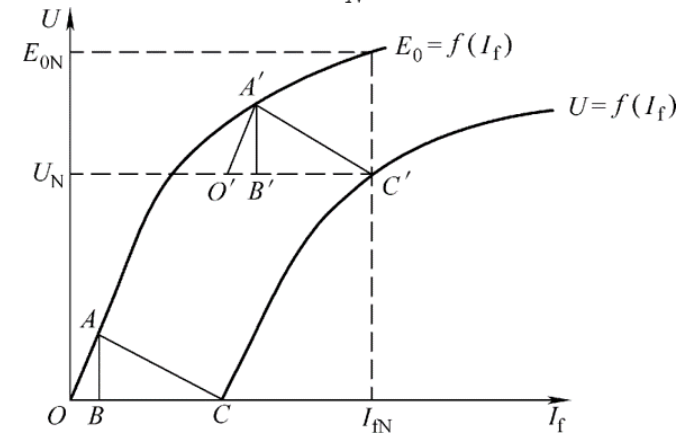
\includegraphics[scale=0.4]{Screenshot_2018-11-05-19-31-43-1997072867.png}
	\captionof{figure}{零功率因数负载特性与空载特性}                   
	\end{center}  
\section{稳态参数的实验测定——转差法测定凸极同步发电机的$x_d$和$x_q$不饱和值}
励磁绕组开路(或通过很大的阻值短路,以防过电压),使{\color{thid}$I_f=0$},用外力拖动转子转动,使{\color{thid}$n\to n_1$(所以转子和定子旋转磁场之间有相对运动}),因此旋转磁场的轴线将不断地依次和转子$d$轴或$q$轴重合,相应地,定子的电抗将随着旋转磁场与转子主磁极相对位置的变化,在最大值$x_d$和最小值$x_q$之间作周期性的变化。\\
\indent 当磁场轴线与转子$d$轴重合时,磁阻最小,定子电抗达最大值$x_d$,而定子电流为最小值$I_{min}$,由于供电线路压降最小,故定子每相的端电压此时为最大值$U_{max}$,忽略定子电阻,则
$$x_{d\text{(不饱和值)}}=\frac{U_{max}}{I_{min}}$$
\indent 同理,当磁场轴线与转子$q$轴重合时,磁阻最大,定子电抗达最小值$x_q$,而定子电流为最大值$I_{max}$,由于供电线路压降最大,故定子每相的端电压此时为最小值$U_{min}$,忽略定子电阻,则
$$x_{q\text{(不饱和值)}}=\frac{U_{min}}{I_{max}}$$
\section{同步发电机的运行特性}
\subsection{外特性——$U=f(I)$}
$n=n_1$,$I_f=\rm{const}$,$\cos\varphi=\rm{const}$时,$U=f(I)$
\begin{itemize}
	\item 感性负载和纯阻性负载时,外特性是下降的。\\
	原因:电枢反应去磁作用+漏阻抗压降
	\item 容性负载且功率因数角为超前时,外特性可能上升。\\
	原因:电枢反应助磁作用+容性电流漏阻抗压降
	\item 电压调整率:
	$$\Delta u=\frac{E_0-U_N}{U_N}\times100\%$$
\end{itemize}
	\begin{center}  
	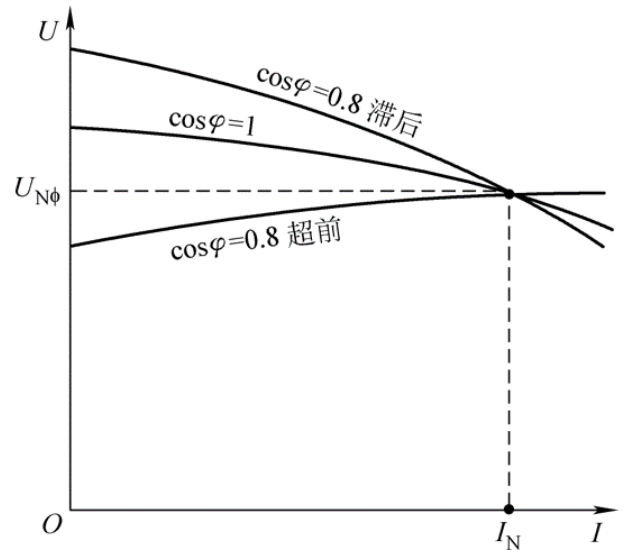
\includegraphics[scale=0.4]{20181105203353.png}
	\captionof{figure}{同步发电机的外特性}                   
	\end{center}  

\subsection{调整特性(与外特性相反)——$I_f=f(I)$}
$n=n_1$,$U=U_N$,$\cos\varphi=\rm{const}$时,$I_f=f(I)$
\begin{itemize}
	\item 感性负载和纯阻性负载时,调整特性上升。
	\item 容性负载且功率因数角为超前时,调整特性可能下降。
\end{itemize}
\subsection{效率特性——$\eta=f(P_2)$}
$n=n_1$,$U=U_N$,$\cos\varphi=\cos\varphi_N$时,$\eta=f(P_2)$

\section{同步发电机电压调整率及额定励磁电流的求取}
从设计的角度看,必须知道从空载到满载时励磁电流变化的范围,这样可以使励磁装置和转子绕组能满足最小和最大励磁电流工作要求。\\
\indent 从运行角度看,也需要知道负载功率因数等与励磁电流的关系。


\chapter{同步发电机并联运行(17)}
\begin{enumerate}
	\item 同步发电机单机供电的缺点:
	\begin{itemize}
		\item 不能保证供电质量(电压和频率稳定问题)h和可靠性(发生故障就得停电)
		\item 无法实现供电的灵活性和经济性
	\end{itemize}
	\item 无穷大电网:$s\to\infty,Z_s\to0,U_s=C,f_s=C$
	\item 单机和并网时调节励磁电流、进水/汽量:
	% Table generated by Excel2LaTeX from sheet 'Sheet1'
	\begin{table}[htbp]
		\centering
		\caption{单机和并网时调节励磁电流、进水/汽量的区别}
		\begin{tabular}{|c|c|c|}
			\hline
			& 励磁电流  & 进水/汽量 \\
			\hline
			单机    & 调节U   & 调节f \\
			\hline
			并网    & 调节无功  & 调节有功 \\
			\hline
		\end{tabular}%
	\end{table}%
	
\end{enumerate}
\section{投入并联运行的条件和方法}
\subsection{投入并联运行的条件——电压相同(五要素)}
$U=U_m\sin(\omega t+\varphi)$+相序【不满足后果:瞬态冲击电流】
\begin{itemize}
	\item 发电机励磁电动势应与电网电压相等($U_m$)
	\item 发电机的频率和电网频率相等($f$)
	\item 并联合闸瞬间,发电机与电网的对应相的电压应同相位($\varphi$)
	\item {\color{thid}相序相同(必须满足)}
	\item 电压波形相同($\sin$)
\end{itemize}
\subsection{同步发电机投入并联的方法}
\begin{enumerate}
	\item 准同步法:{\color{thid}先调节发电机电压与电网电压相等,再通过准同步法调整相位;并网时,频率与电网频率接近,并网后通过\underline{自整步作用}使两者频率相等。}(P.224)
	\begin{itemize}
		\item 手动准同步并列:
		\begin{itemize}
			\item[-] {\color{thid}\underline{灯光熄灭法}}: 三只灯直接跨接到电网与发电机对应相上。
			\begin{itemize}
				\item[*] 并网条件:调节发电机的转速使灯光明暗变化十分缓慢时,说明同步发电机和电网频率十分接近,等待灯光完全变暗的瞬间到来,即可合闸投入并列。
				\item[*] 不同现象:
			% Table generated by Excel2LaTeX from sheet 'Sheet1'
			\begin{table}[htbp]
				\centering
				\caption{不同灯光现象反应的电路状态}
				\begin{tabular}{|c|c|c|c|c|}
					\hline
					序号    & 1     & 2     & 3     & 4 \\\hline
					现象    & 灯同时暗、亮 & 没有完全变暗的时候 & 不同时暗、亮 & 不熄灭 \\\hline
					反映    & f不相等  & 电压不等  & 相序不等  & 相位不等 \\\hline
				\end{tabular}%
			\end{table}%			
			\end{itemize}
			\item[-] {\color{thid}\underline{灯光旋转法}}: 灯1(跨接到A1A2),灯2(跨接到(B1C2),灯3(跨接到C1B2)
				\begin{itemize}
					\item[*] 并网条件:调节发电机的转速使灯光旋转十分缓慢时,说明同步发电机和电网频率十分接近,等待灯光1完全变暗且2、3亮度完全相等的瞬间到来,即可合闸投入并列。
					\item[*] 灯光不旋转说明相序不等
					\item[*] 旋转方向可以用来判定发电机频率和电网频率的大小关系
				\end{itemize}
		\end{itemize}
		\item 半自动准同步并列
		\item 自动准同步并列
	\end{itemize}
	\item 自同步法{\color{thid}(用于事故状态下并车)}:励磁电流通过电阻$r_m$(约为励磁电阻的10倍)短接,拖动到接近同步转速(相差$2\%\sim5\%$),在无励磁电流的情况下,将发电机接入电网。再接通励磁并调节励磁,依靠定子磁场和转子磁场之间的电磁转矩将转子拉入同步,并列过程结束。{\color{blue}(在接入励磁电源之前,励磁绕组必须通过一限流电阻构成闭合回路)}
	\begin{note}
		因为直接开路,将在其中感应出危险的高压;直接短路,将在定、转子绕组间产生很大的冲击电流。	
	\end{note}
\end{enumerate}

\section{并网运行的同步发电机的电磁功率与功角特性}
\subsection{同步发电机的功率与转矩平衡}
\begin{enumerate}
	\item 功率流程:\\
		$P_1$为原动机向发电机的输入机械功率;提供轴与轴承之间的摩擦、转动部分与空气的摩擦及通风设备的损耗总计为机械损耗$p_m$和杂散损耗$p_s$;供给{\color{red}\underline{定子铁心}中的涡流和磁滞损耗},总计为{\color{red}铁心损耗$p_{Fe}$};$P_{em}$为通过电磁感应作用转换为定子绕组上的电功率。称为电磁功率。如果是负载运行,定子绕组中还存在定子铜耗$p_{cu1}$;$P_2=P_{em}-p_{cu1}$为发电机输出功率。励磁回路所消耗的电功率一般由原动机或其他电源供给,故不包括在功率流程中,同步发电机的功率平衡方程式为:
		\begin{displaymath}
			\begin{aligned}
				P_{1\phantom{b1}} &= P_{em}+p_{Fe}+p_m+p_s\\
				P_{em} &= P_2+p_{cu1}
			\end{aligned}
		\end{displaymath}
		\begin{center}  
			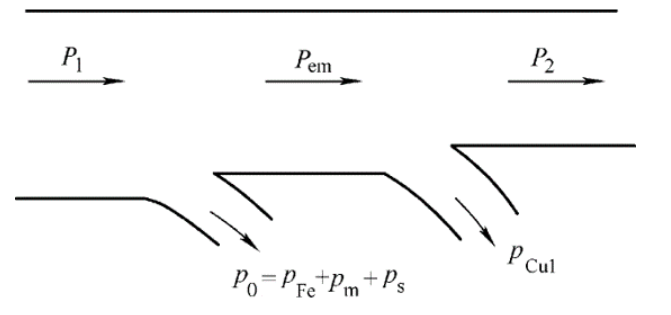
\includegraphics[scale=0.4]{20181108160804.png}
			\captionof{figure}{同步发电机的功率流程}
		\end{center}  
	\item 定子绕组的电阻一般较小其铜耗$p_{cu1}$可以忽略不计,则有:
	$$P_{em}=P_2=mUI\cos\varphi$$
	\item 转矩平衡式:
	$$T_1=T_0+T$$
	$T_1=\frac{P_1}{\Omega_1}$为发电机轴上的输入机械转矩;$T_0=\frac{P_0}{\Omega_1}$为空载轴上的输入转矩;$T=\frac{P_{em}}{\Omega_1}$为电磁转矩,$\Omega_1=\frac{2\pi n_1}{60}(rad/s)$。
\end{enumerate}
\subsection{隐极发电机的功率特性(有功特性)与转矩特性}
\begin{enumerate}
	\item 功角特性:并联于无穷大电网的同步发电机,当电网电压和频率恒定、参数为常数、空载电动势$E_0$不变(即$I_f$不变)时,电磁功率和功率角($E_0$和$U$的夹角)之间的关系$P_{em}=f(\delta)$称为有功功率特性,也称功角特性。对于隐极发电机,有$$\boxed{P_{em}=\frac{mE_0U}{x_s}\sin\delta}$$
	\begin{note}
		$\delta$的物理意义:转子磁场轴线和定子合成磁极轴线的空间夹角
	\end{note}	

	\begin{figure}[!hbtp]
		\centering
		\subfigure[隐极发电机的时空相矢图]{
			\begin{minipage}{0.35\textwidth}
				\centering
				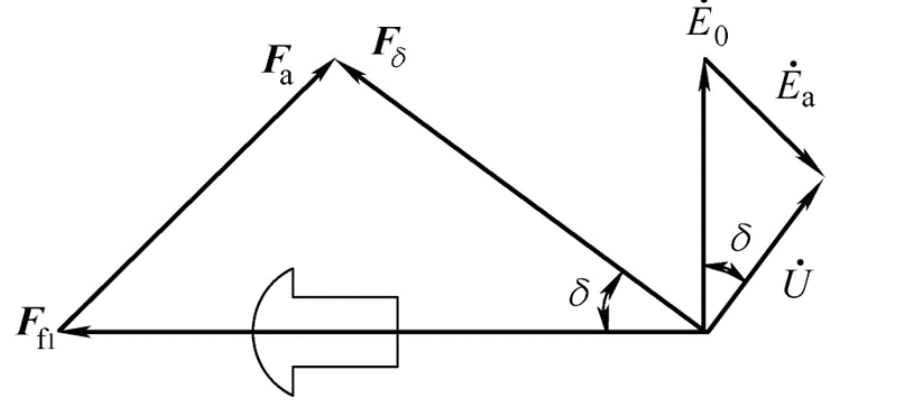
\includegraphics[scale=0.2]{20181108165449.png}
			\end{minipage}
		}
		\subfigure[功角的空间模型]{
			\begin{minipage}{0.3\textwidth}
				\centering
				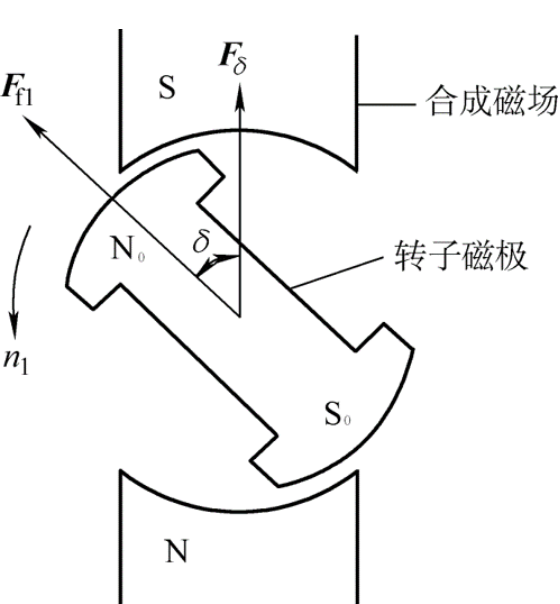
\includegraphics[scale=0.2]{20181108165505.png}
			\end{minipage}
		}
	    \subfigure[功率特性]{
	    	\begin{minipage}{0.3\textwidth}
	    		\centering
	    		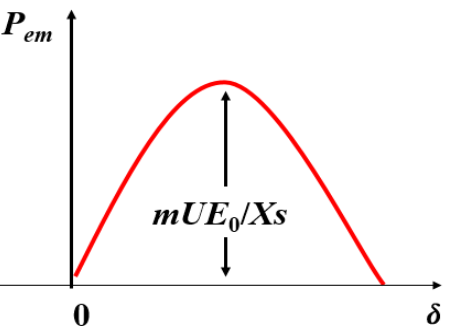
\includegraphics[scale=0.25]{20181108170721.png}
	    	\end{minipage}
	    }
		\caption{隐极同步发电机磁路不饱和时等效电路,向量图和功率特性}      
	\end{figure}
		\item 转矩特性:忽略电枢电阻,则得电磁转矩的公式为
		$$T=\frac{P_{em}}{\Omega}=\frac{p}{\omega}\frac{E_0}{x_s}\sin\delta$$	
		在用标幺值表示时,由于取速度的基值为同步转速,所以同步发电机正常运行时转速标幺值为1,转矩和功率有相同标幺值
\end{enumerate}
\subsection{凸极发电机的功率特性(有功特性)}
	\begin{displaymath}
	\begin{aligned}
			P_{em} &= \frac{mE_0U}{x_d}\sin\delta+mU^2(\frac{1}{x_q}-\frac{1}{x_d})\sin\delta\cos\delta\\
			&=\frac{mE_0U}{x_d}\sin\delta+mU^2\frac{x_d-x_q}{2x_dx_q}\sin2\delta\\
			&= {P_{em}}\rq+{P_{em}}^{''}
	\end{aligned}                                     
	\end{displaymath}
\begin{itemize}
	\item 第一项${P_{em}}\rq$为基本电磁功率,由于${P_{em}}\rq\propto E_0$,所以又称为励磁功率,是定子电流与转子磁场之间的相互作用形成的。
	\item
	第二项${P_{em}}^{''}$为附加电磁功率,它由d、q轴磁导差异而产生的,又称磁阻功率,与励磁无关,只与电网电压有关。
	\item 无论凸极机、隐极机,当功角$\delta=0$时,$P_{em}$都为0。
\end{itemize}
\subsection{无功功率与功角关系}
\begin{enumerate}
	\item 隐极机:$$Q=\frac{mE_0U}{x_s}\cos\delta-\frac{mU^2}{x_s}$$
	\begin{center}  
		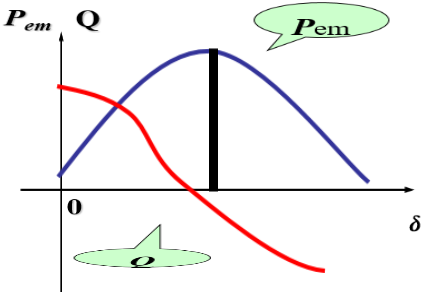
\includegraphics[scale=0.4]{20181108204503.png}
		\captionof{figure}{隐极同步发电机的有功功率和无功功率特性}
	\end{center}  
	\begin{itemize}
		\item $Q>0$,发出感性无功(吸收容性无功)
		\item $Q=0$,$\delta<90\degree$
		\item $Q<0$,吸收感性无功(发出容性无功)
	\end{itemize}
	\item 凸极机:$Q=\frac{mE_0U}{x_d}\cos\delta-\frac{mU^2}{2}(\frac{1}{x_q}+\frac{1}{x_d})+\frac{mU^2}{2}(\frac{1}{x_q}-\frac{1}{x_d})\sin2\delta$({\underline{不用记}})
\end{enumerate}
\section{并网运行时有功功率的调节与静态稳定}
\subsection{有功功率的调节}
{\color{thid}要改变有功功率,需要改变原动机提供的驱动转矩。}以隐极同步发电机为例,刚并网的发电机,$\dot{E_0}=\dot{U},\delta=0,P_2=P_{em}=0,P_1=P_0$,处于平衡状态,此时发电机输出的有功功率$P_2\approx P_{em}=\frac{mE_0U}{x_s}\sin\delta=0$。增加输入机械功率$P_1$,假设保持励磁电流不变,则$P_1>P_0$,$P_1-P_0>0$,发电机处于加速过渡过程,转子加速,转子磁场位置将超前合成磁场,$\delta>0$。随着$\delta$增加,$P_2=P_{em}>0$增加,当达到新的平衡$P_1-P_0=P_{em}$时,加速过程结束,进入稳态运行,机械功率转换成电磁功率,使发电机输出有功功率,达到新的功率平衡。电磁功率最大值也称功率极限:
$$P_{em\phantom{a}max}=\frac{mE_0U}{x_s}$$
在功率极限范围内,输入功率越大,有功功率输出就越大。
\begin{note}
	可以得知,$I_f\uparrow$,$x_s\downarrow$(气隙增大),都可以使$P_{em}$增大;所以,并网运行时不希望气隙小。而气隙越小,需要的励磁电路越小。所以,同步发电机的气隙不能太大,也不能太小。
\end{note}
\subsection{静态稳定}
\begin{enumerate}
	\item 静态稳定和动态稳定:
		\begin{itemize}
			\item 静态稳定:并联在电网上稳定运行的同步发电机,当受电网或原动机方面\underline{某些微小扰动}时,如果不考虑调压器和调速器的作用,发电机能自动恢复到原来运行状态。
			\item 动态稳定:同步发电机遇到突然加负载、切除负载等正常操作,或者发生短路、电压突变、发电机发生励磁电流等非正常运行时,发电机能否继续保持同步运行的问题。
		\end{itemize}
	\item 隐极发电机的静态稳定问题:\\
	$0\leq\delta<90\degree$,静态稳定。
		\begin{center}  
			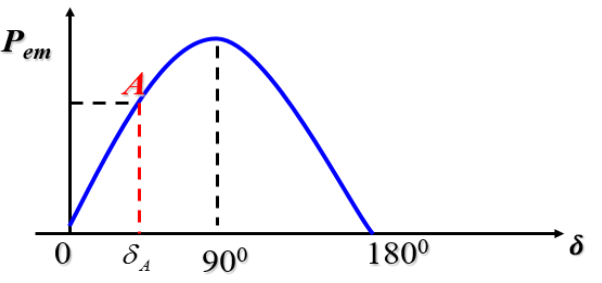
\includegraphics[scale=0.4]{20181108220518.png}
			\captionof{figure}{静态稳定}
		\end{center}  
		\begin{itemize}
			\item 比整步功率:
			$$P_{syn}=\frac{dP_{em}}{d\delta}=m\frac{E_0U}{x_s}\cos\delta$$
			\item 过载能力:
			$$K_m=\frac{P_{em\phantom{a}max}}{P_N}\approx \frac{1}{\delta_N}$$	
			\item 远距离输电时:\\
			为提高远距离输电的静态稳定,除系统中采取措施外,从发电机角度来说,希望发电机有较小的同步电抗,也就是要有较大的短路比。
			\begin{note}
			\underline{若发电机经变压器及输电线与电网并联,则相当于$x_s$改为$(x_s+x_T+x_L)$} ,其中$x_T$是变压器的短路电抗,$x_L$为输电线路电抗。且都是折算到发电机侧的数值。这时,发电机的最大电磁功率为$P_{em\ s max}=mE_0U/(x_s+x_T+x_L)$,\underline{显然过载能力降低了,特别是线路较长时,对稳定运行很不利。}
			\end{note}
		\end{itemize}
\end{enumerate}
\section{并网运行时无功功率的调节与$V$形曲线}
\subsection{无功功率的调节}
\begin{enumerate}
	\item 无功功率的调节必须依靠励磁电流的调节
	\begin{note}	
	并网的同步发电机一般在向系统输出{\color{thid}有功功率}的同时,也向系统输出{\color{thid}感性无功功率。}此时,发电机的电枢反应在直轴方向是{\color{thid}去磁性质}。为了维持发电机端电压不变,必须增加励磁电流。
	\end{note}	
	\item 可以单独调节无功功率,但是做不到单独调节有功功率
	\begin{note}
	当发电机的励磁电流不变时,$\delta$的变化将使无功功率发生变化。感性无功功率随着有功功率的增加而减少,甚至可能导致无功功率改变性质。因此,如果只要求改变发电机所承担的有功功率时,应该在调节发电机有功功率的同时,适当调节发电机的励磁电流。
	\end{note}
	\item	负载和有功输入不变时,同步发电机输出的有功功率不变
	\begin{note}
		功率平衡
	\end{note}
	\item	三种励磁情况
	\begin{center}
		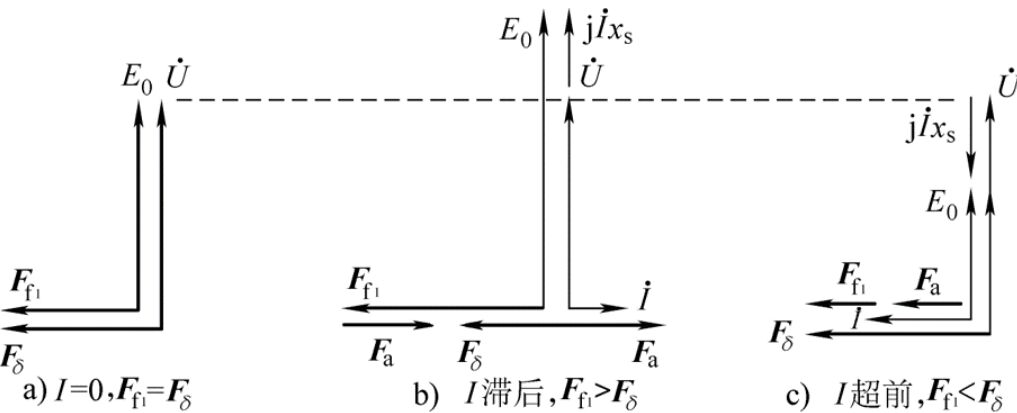
\includegraphics[scale=0.3]{20181115164133.jpg}
		\captionof{figure}{无功输出为零不同励磁的时空相矢图}
	\end{center}
	\begin{itemize}
		\item 正常励磁:
		\begin{itemize}
			\item [*]未带有功负载(i.e.刚并网的同步发电机)
			\item [*] 励磁电动势=端电压,即$\dot{E_{0}}=\dot{U}$,电枢电流为0,且不存在电枢磁动势,励磁绕组的主磁动势$F_{f1}$与合成磁动势$F_{\delta}$相等
			\item [*] 发出无功=0	
		\end{itemize}
		\item 过励磁:
		\begin{itemize}
			\item[*]  $\dot{E_{0}}=\dot{U}+j\dot{I}x_s$
			\item[*] 去磁,$F_{\delta}=F_{f}-F_{a}$	
			\item[*] 发出感性无功
		\end{itemize}
		\item 欠励磁:
		\begin{itemize}
			\item[*]  $\dot{E_{0}}=\dot{U}+j\dot{I}x_s$
			\item[*] 助磁,$F_{\delta}=F_{f}+F_{a}$	
			\item[*] 发出容性无功
		\end{itemize}
	\end{itemize}
\end{enumerate}
\subsection{$V$形曲线}
	\begin{center}
		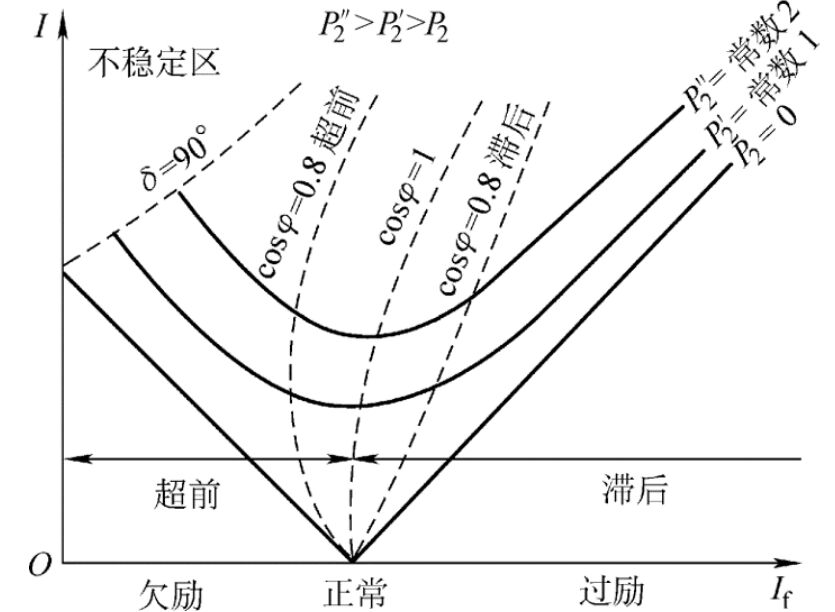
\includegraphics[scale=0.3]{20181115165555.jpg}
		\captionof{figure}{同步发电机的$V$形曲线}
	\end{center}
\begin{itemize}
	\item 不稳定区域边缘:$\delta=90\degree$(左边界),连线向右倾斜
	\item	每条曲线上的电流变化量$\Delta I$为无功分量
	\item 	欠励磁时,励磁电流增大,电枢电流变化规律为为先减小后增大。
	\item 有功功率越大,$V$形曲线越高
	\item	每条曲线最低点$\cos\varphi=1$,定子电流最小,不管励磁电流增加或减小,定子电流都将增大
	\item	励磁电流增大受绕组最大允许电流限制(右边界),电流过大,电枢绕组会过热损坏
	\item	各$V$形曲线最低点连接线为$\cos\varphi=1$的曲线,该连线向右倾斜。{\color{blue}因为随有功功率增加,$Ix_s$也增加,需相应增加励磁电流,以维持$\cos\varphi=1$}
\end{itemize}
\section{*同步发电机的振荡}
\begin{itemize}
	\item 同步发电机的振荡:\\
	当负载突然变化时,由于转子有惯性,转子功角不能立即稳定在新的数值,而是要在新的稳定值左右经过若干次摆动。
	\item 为使振荡能尽快趋于稳定,通常在转子表面装设{\color{blue}阻尼绕组}
\end{itemize}


\chapter{同步发电机的异常运行(18)}
\section{同步发电机的不对称运行}
第我国2009年颁布的标准GB755-2008《旋转电机$\ $定额和性能》
第7.2.2条规定:负序和零序电流分量均不超过正序分量的5\%
\subsection{相序阻抗和等效电路}
\begin{enumerate}
	\item 正序阻抗:转子通入励磁电流正向同步旋转时,电枢绕组的{\color{blue}正序}三相对称电流所遇到的阻抗。{\color{red}正序阻抗=对称运行时的阻抗}
	\item 负序阻抗:转子正向同步旋转,但{\color{red}励磁绕组短路}(因为不存在负序励磁电动势:{\color{blue}空载电动势对称,电流不对称是由负载不对称引起}),电枢绕组的{\color{blue}负序}三相对称电流所遇到的阻抗
	\begin{itemize}
		\item	电枢电流产生反向圆形旋转磁场$F_{-}$,方向与转子转向相反,速度为$n_1$,即以$2n_1$切割转子,在转子中产生感应电动势和电流,且频率为$f_2=pn/60=2f_1$
		\item 转子绕组对定子绕组的影响可以看成异步电机转子堵转时对定子绕组的影响(对交流电而言,发电机转子绕组相当于短路),这样类似于异步电机堵转时的等效电路。
		\begin{note}
		将转子励磁绕组、阻尼绕组及转子本身看成以一对称的 多相短路绕组,转子电流流入转子绕组产生的旋转磁场$F_2$,相对转子的速度为$2n_1$,可见,$F_2$与$F_{-}$相对静止。	
		\end{note}
		\item 4个阻抗值:
		由于电阻值远小于电抗值,故可略去不计。
		\begin{itemize}
			\item[*] 	直轴上有阻尼绕组时,有直轴次暂态电抗$x_d^{''}$
			$$x_{d-}=x_{\sigma}+\frac{1}{\frac{1}{x_{ad}}+\frac{1}{x_{f\sigma}}+\frac{1}{x_{D\sigma}}}=x_d^{''}$$
			\item[*] 	直轴上无阻尼绕组时,有直轴暂态电抗$x_d^{'}$
			$$x_{d-}=x_{\sigma}+\frac{1}{\frac{1}{x_{ad}}+\frac{1}{x_{f\sigma}}}=x_d^{'}$$
			\item[*] 	交轴上没有励磁绕组,但有交轴阻尼绕组时,有交轴次暂态电抗$x_q^{''}$
			$$x_{d-}=x_{\sigma}+\frac{1}{\frac{1}{x_{aq}}+\frac{1}{x_{D\sigma}}}=x_d^{'}$$
			\item[*] 	交轴上没有阻尼绕组时,有
			$$x_{q-}=x_{\sigma}+x_{aq}=x_q$$
		\end{itemize}
	\end{itemize}

	\item 零序阻抗:转子正向同步旋转,但{\color{red}励磁绕组短路},电枢绕组的{\color{blue}零序}电流(同大小、同相位)所遇到的阻抗
	\begin{note}
	一般不考虑零序分量,因为励磁绕组一般是"Y"型联结,零序电流流不动,所以建立的合成磁动势为0。{\color{red}零序电抗基本等于定子漏抗,$x_0\approx x_{\sigma}$}	
	
	\item 各序等效电路
	\begin{center}
		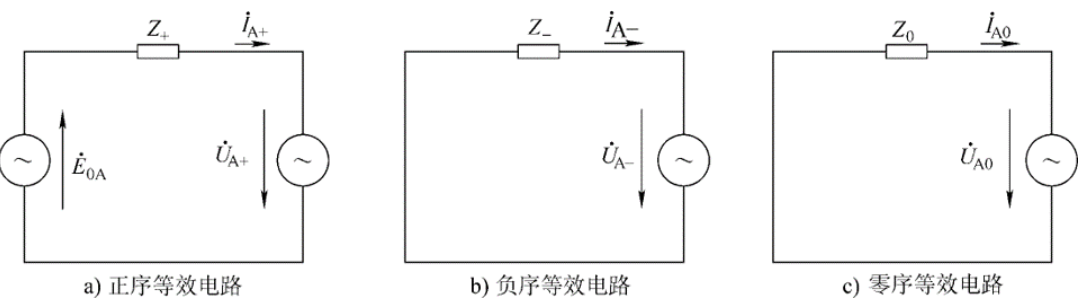
\includegraphics[scale=0.35]{Screenshot_2018-11-23-14-14-44-1965787396.png}
		\captionof{figure}{各相序等效电路}
	\end{center}
	\end{note}
\end{enumerate}

\subsection{同步发电机不对称运行分析实例}
\indent 在发生故障短路时,整个过程一般分为两个阶段:
\begin{enumerate}
	\item 突然短路:此阶段产生很大的冲击电流,经过零点几秒到几秒时间,此冲击电流将逐渐衰减完毕,然后进入第二阶段,即稳态短路阶段。
	\item 稳态短路阶段:稳态短路时短路电流将受到线路阻抗的限制,此电流的有效值一般是恒定的。
\end{enumerate}
为简化分析,通常假设短路前处于空载状态和短路点发生在发电机的出线端,下面分析单相对中性点稳态短路和两相线间稳态短路两种情况。
\begin{enumerate}
	\item 单相点对中性点(单相对地短路)稳态短路
	\begin{itemize}
		\item 边界条件:
		\begin{displaymath}
		\begin{aligned}
			\dot{U}_A&=0\\
			\dot{I}_A&=\dot{I}_{k1}\\
			\dot{I}_B&=\dot{I}_C=0
		\end{aligned}
		\end{displaymath}
		\item 利用对称分量法求出相序分量:
		\begin{displaymath}
		\begin{aligned}
			\dot{U}_A&=\dot{U}_{A+}+\dot{U}_{A-}+\dot{U}_{A0}=0\\
			\dot{I}_{A+}&=\frac{\dot{I}_{A}+\alpha \dot{I}_{B}+\alpha^{2}\dot{I}_{C}}{3}=\frac{1}{3}\dot{I}_{A}\\
			\dot{I}_{A-}&=\frac{\dot{I}_{A}+\alpha^{2} \dot{I}_{B}+\alpha\dot{I}_{C}}{3}=\frac{1}{3}\dot{I}_{A}\\
			\dot{I}_{A0}&=\frac{\dot{I}_{A}+ \dot{I}_{B}+\dot{I}_{C}}{3}=\frac{1}{3}\dot{I}_{A}
		\end{aligned}
		\end{displaymath}
		然后利用相序等效电路及电动势方程求解如下:
		\begin{displaymath}
		\begin{aligned}
			\dot{E}_0&=\dot{U}_{A+}+\dot{I}_{A+}Z_{+}\\
			0&=\dot{U}_{A-}+\dot{I}_{A-}Z_{-}\\	
			0&=\dot{U}_{A0}+\dot{I}_{A0}Z_{0}\\	
		\end{aligned}
		\end{displaymath}
		上面三式相加,整理得到:
		$$\dot{I}_{A+}=\frac{\dot{E}_{0}}{Z_{+}+Z_{-}+Z_{0}}$$
		所以,所求单相短路电流$\dot{I}_{k1}$:
		$$\dot{I}_{k1}=3\dot{I}_{A+}=\frac{3\dot{E}_{0}}{Z_{+}+Z_{-}+Z_{0}}$$
		\begin{center}
			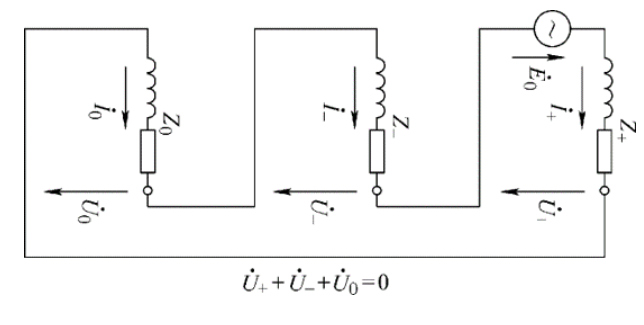
\includegraphics[scale=0.4]{Screenshot_2018-11-23-14-19-27-0048381808}
			\captionof{figure}{单相短路等效电路}
		\end{center}
		\begin{note}
			因为电路中$\dot{I}_{A+}=\dot{I}_{A-}+\dot{I}_{A0}$,所以要把三序等效电路串联起来
		\end{note}
		\end{itemize}
	
	\item 两相线间稳态短路\\
	$C\text{、}B$线间发生短路,$A$相保持空载。
	\begin{itemize}
		\item 边界条件:
		\begin{displaymath}
		\begin{aligned}
		\dot{U}_{BC}&=0\text{,即}\dot{U}_{B}=\dot{U}_{C}\\
		\dot{I}_A&=0\\
		\dot{I}_{k2}&=\dot{I}_{B}=-\dot{I}_C
		\end{aligned}
		\end{displaymath}
		\item 利用对称分量法求出相序分量:
		\begin{displaymath}
		\begin{aligned}
			\dot{I}_{A+}&=\frac{\dot{I}_{A}+\alpha \dot{I}_{B}+\alpha^{2}\dot{I}_{C}}{3}=\frac{1}{3}(\alpha-\alpha^{2})\dot{I}_{k2}=j\frac{1}{\sqrt{3}}\dot{I}_{k2}\\
			\dot{I}_{A-}&=\frac{\dot{I}_{A}+\alpha^{2} \dot{I}_{B}+\alpha\dot{I}_{C}}{3}=\frac{1}{3}(\alpha^{2}-\alpha)\dot{I}_{k2}=-j\frac{1}{\sqrt{3}}\dot{I}_{k2}\\
			\dot{I}_{A0}&=\frac{\dot{I}_{A}+ \dot{I}_{B}+\dot{I}_{C}}{3}=0
		\end{aligned}
		\end{displaymath}
	    由于有
	    \begin{displaymath}
	    \begin{aligned}
		    \dot{U}_{B}&=\dot{U}_{B+}+\dot{U}_{B-}+\dot{U}_{B0}=\alpha^{2}\dot{U}_{A+}+\alpha\dot{U}_{A-}+\dot{U}_{A0}\\
		    \dot{U}_{C}&=\dot{U}_{C+}+\dot{U}_{C-}+\dot{U}_{C0}=\alpha\dot{U}_{A+}+\alpha^{2}\dot{U}_{A-}+\dot{U}_{A0}\\
		    \dot{U}_{B}&=\dot{U}_{C}
	    \end{aligned}
	    \end{displaymath}
	    所以,{\color{blue}$\boxed{\dot{U}_{A+}=\dot{U}_{A-}}$}
	    然后利用相序等效电路及电动势方程求解如下:
		\begin{displaymath}
		\begin{aligned}
		\dot{E}_0&=\dot{U}_{A+}+\dot{I}_{A+}Z_{+}\\
		0&=\dot{U}_{A-}+\dot{I}_{A-}Z_{-}\\	
		0&=\dot{U}_{A0}+\dot{I}_{A0}Z_{0}\\	
		\end{aligned}
		\end{displaymath}
		整理得到:
		$$\dot{I}_{A+}=-\dot{I}_{A-}=\frac{\dot{E}_{0}}{Z_{+}+Z_{-}}$$
		所以,所求两相线间稳态短路电流$\dot{I}_{k2}$:
		$$\dot{I}_{k2}=-j\sqrt{3}\dot{I}_{A+}=-j\frac{\sqrt{3}\dot{E}_{0}}{Z_{+}+Z_{-}}$$
		\begin{center}
			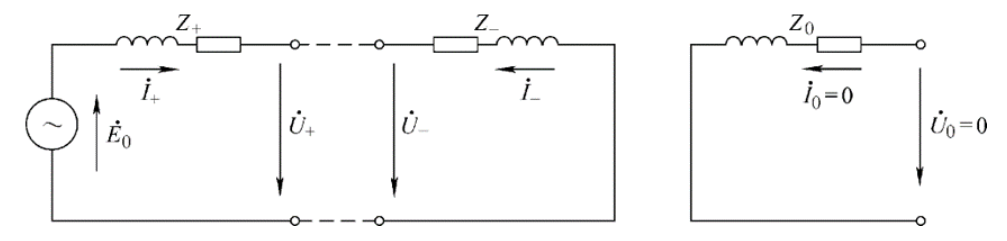
\includegraphics[scale=0.35]{Screenshot_2018-11-23-14-22-50-1086542749.png}
			\captionof{figure}{线间短路等效电路}
		\end{center}
		\begin{note}
			对于零序系统,线间短路无中性线,不存在零序系统
		\end{note}
	\end{itemize}
	\item 不同稳态短路电流的比较
		\begin{note}
			负序阻抗和零序阻抗$\ll$正序阻抗,三相稳态短路是对称的$\Longrightarrow$  $$\dot{I}_{k1}\approx \frac{3\dot{E}_{0}}{Z_{+}}=3\dot{I}_{k3}$$所以,单相稳态短路电流$\dot{I}_{k1}>\text{三相稳态短路电流}\dot{I}_{k3}$,同理可得:$$I_{k1}:I_{k2}:I_{k3}=3:\sqrt{3}:1$$
		\end{note}	
\end{enumerate}
\subsection{不对称运行对发电机的危害}
\indent	不对称运行对发电机的危害主要有2点:
	\begin{enumerate}
		\item 转子表面局部过热而发生转子烧损事故
			\begin{itemize}
				\item 三相电流不对称时,由于转子结构不对称,负序对称电流分量在转子各部件上感应的2倍工频电流分布不均,容易出现局部温度升高、过热
				\item 感应产生的2倍工频电流,不仅沿转子轴向分布,还沿径向分布,形成环流,电流流经护环及其嵌装表面等部位时,因各部位的接触电阻较大,也容易出现高温和过热
			\end{itemize}
		\item 转子产生振动,进而发生轴瓦磨损
			\begin{itemize}
				\item 负序磁场以2倍同步转速切割转子及转子本身,磁路不对称,在定转子之间产生交变的电磁转矩,致使转子受的力矩也是交变的
				\item 转子上的2倍工频电流流经转子上各部件,因其使用材料不同,各自的热容量也不同,如护环的热容量较小,在护环与转子本体之间就会形成温差,使护环失去紧力;失去紧力后,因径向位移量很小,不会在轴上自由回转,但在不平衡力作用下,护环可能一侧紧贴转子轴表面,而另一侧稍离转子表面,使转子中心偏移,转子产生振动
				\item 负序电流在转子表面局部产生高温过热,转子受热不均,发生不对称变形也可能使转子产生振动
			\end{itemize}
	\end{enumerate}
\section{同步发电机突然短路时的暂态电抗}
\indent	发电机从原来的稳态运行状态过渡到稳态短路状态,该过渡过程包括次暂态(有阻尼绕组)、暂态和稳态短路3个阶段。
\begin{note}
突然短路时,定子电流在数值上发生急剧变化,电枢反应磁通也随着变化,并在转子的励磁绕组和阻尼绕组中感应电动手机和感应电流,这些电流将各自建立各自的磁场,又反过来影响电枢磁场和定子电流的变化。这种定子和转子绕组之间的互相影响,致使在短路过程中,定子绕组的电抗<稳态同步电抗,从而导致在短路过程中,定子短路电流很大,并且是一个随时间衰减的电流。
\end{note}
如果{\color{blue}发生三相突然短路},那么
\begin{enumerate}
	\item 直轴次暂态电抗$x_d^{''}$
	\begin{itemize}
		\item 
		发生三相突然短路时,由于电枢电流和电枢磁链的突然变化,突然变化的磁链$\varPsi_{ad}$要穿过转子绕组,但{\color{blue}励磁绕组和阻尼绕组交链的磁链不能突变},故要感应出电流,抵消突变部分磁链$\varPsi_{ad}$的变化,从而维持传过自己的磁链不变。
		\item 所以相当于$\varPsi_{ad}$被挤出,只能从阻尼绕组和励磁绕组外侧的漏磁路通过,成为次暂态磁链$\varPsi^{'}_{ad}$
		\item 对应有直轴次暂态电抗$x_d^{''}=x_{ad}^{''}+x_{\sigma}$,其中
		$$x_{ad}^{''}=\frac{1}{\frac{1}{x_{ad}}+\frac{1}{x_{f\sigma}}+\frac{1}{x_{d\sigma}}}$$
	\end{itemize}
	\item 直轴暂态电抗$x_d^{'}$
	\begin{itemize}
		\item 由于同步发电机各绕组都有电阻存在,因此阻尼绕组和励磁绕组中短路引起的感应电流分量都会随时间衰减为0
		\item 阻尼绕组匝数少,电感小,时间常数大,电流很快衰减为0。
		\item 所以可以近似认为阻尼绕组中感应电流衰减完之后,励磁绕组电流分量才开始衰减。
		\item 此时电枢磁链可穿过阻尼绕组,但被挤在励磁绕组外侧的漏磁路上,成为暂态磁链$\varPsi^{'}_{ad}$,发电机进入暂态过程。
		\item 此时磁路包括气隙磁阻、励磁绕组漏磁路磁阻,因此有对应的直轴暂态电抗$x_d^{'}=x_{ad}^{'}+x_{\sigma}$,其中
		$$x_{ad}^{'}=\frac{1}{\frac{1}{x_{ad}}+\frac{1}{x_{f\sigma}}}$$
	\end{itemize}
	\item 直轴同步电抗$x_d$
	\begin{itemize}
		\item 在励磁绕组中的感应电流也衰减完后,只有励磁绕组$I_f$存在,电枢磁链穿过阻尼绕组和磁绕组,发电机进入稳态短路过程,过渡过程结束。
		\item 这时对应直轴同步电抗$x_d=x_{ad}+x_{\sigma}$
	\end{itemize}	
\end{enumerate}
如果{\color{blue}通过负载短路},那么
	\begin{itemize}
		\item 短路电流产生的电枢磁场不仅有直轴分量,还会有交轴分量。
		\item 由于交轴方向没有励磁绕组,交轴方向的磁路和电抗与直轴的有所不同。
		\item 交轴次暂态电抗$x_q^{''}=x_{aq}^{''}+x_{\sigma}$,其中
		$$x_{aq}^{''}=\frac{1}{\frac{1}{x_{aq}}+\frac{1}{x_{D\sigma}}}$$
		\item 交轴暂态电抗$x_q^{'}=x_{aq}^{'}+x_{\sigma}=x_q$,由于没有励磁绕组,$x_{aq}^{'}=x_{aq}$
	\end{itemize}

\chapter{同步电动机(19)}
定义$F_{\delta}$超前$F_{f}$时,$\delta>0$。所以分析时,将同步发电机的表达式中的$\delta$变为$-\delta$

\chapter{直流电机的基本工作原理与结构(20)} 
\section{直流电机的基本工作原理}
\indent 一般直流电机是磁极固定,{\color{thid}电枢旋转}的结构。{\color{thid}一台直流电机原则上既可以作为电动机运行,也可以作为发电机运行。}
\begin{enumerate}
	\item 直流发电机:\\
	直流发电机运行时电枢线圈内电动势、电流方向是交流电,电刷间为直流电动势,线圈中感应电动势与电流方向一致,产生的电磁转矩方向$T$方向由左手定则判断,与转子转向\underline{相反},\underline{制动}性质。
	\\{\color{red}在换相片上放置着一对固定不动的电刷A和B,这样保证了$U_{AB}>0$}
		\begin{figure}[!hbtp]
			\centering
			\subfigure[直流发电机物理模型]{
				\begin{minipage}{0.35\textwidth}
					\centering
					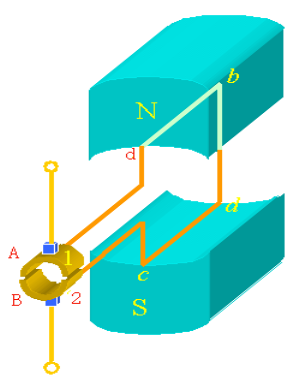
\includegraphics[scale=0.5]{1244.PNG}
				\end{minipage}
			}
			\subfigure[直流发电机原理]{
				\begin{minipage}{0.3\textwidth}
					\centering
					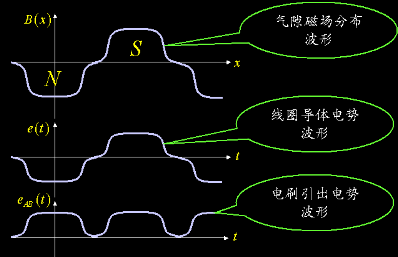
\includegraphics[scale=0.7]{12344.PNG}
				\end{minipage}
			}\caption{直流发电机物理模型及原理}      
		\end{figure}
		\\为了得到稳定的直流电势,直流电机的电枢圆周上一般有多个线圈分布在不同的位置,
		并通过多个换向片联接成电枢绕组。
	\item 直流电动机\\
		外加的电源是直流的,但由于电刷和换相片的作用,在线圈中流过的电流是交流的,其产生的转矩方向却是不变的。
\end{enumerate}
\section{直流电机的基本结构}
\begin{center}
	\includegraphics[scale=1]{zldj_structure.png}
	\captionof{figure}{直流电机的基本结构}
\end{center}
\section{直流电机的额定值与型号}
额定功率$P_{N}$指输出的功率
\begin{itemize}
	\item 对于直流发电机,$P_{N}$指输出的\colorbox{pink}{电}功率
	\item	对于直流电动机,$P_{N}$指输出的\colorbox{pink}{机械}功率
\end{itemize}


\chapter{直流电机的运行原理(21)}
\begin{center}
	\includegraphics[scale=0.6]{zldj _zcjhl1.png}
	\captionof{figure}{直流电机主磁极回路}
\end{center}
\section{直流电动机空载运行磁场}
\begin{enumerate}
	\item 磁通与磁动势:
	\begin{itemize}
		\item 主磁通$\Phi_0$:同时交链励磁绕组和电枢绕组。
		\begin{itemize}
			\item 主磁通路径:主磁极(N极)、气隙、电枢齿、电枢铁心、电枢齿、气隙、另一主磁极(S极)、定子磁轭回到主磁极(N极)。
			\item 功能:随电枢旋转产生感应电动势和电磁转矩,参与机电能量转换,是\colorbox{pink}{工作磁通}
		\end{itemize}
		\item 漏磁通$\Phi_{\sigma}$:\colorbox{pink}{仅交链励磁绕组},不交链电枢绕组。
		\begin{itemize}
			\item 不穿过电枢表面,\colorbox{pink}{不参加机电能量转换}
			\item 漏磁路气隙大,磁阻大,漏磁通比主磁通小得多。
		\end{itemize}
	\end{itemize}
	\item	主磁场的分布:\\
	不考虑电枢表面齿槽效应,假设电枢表面光滑,气隙磁动势为$F_{\sigma}$,$x$处的气隙长度为$\sigma(x)$,空载时的磁密用函数$B_{0}(x)$表示,根据磁路定律有$B_{0}(x)=\mu _{0}F_{\delta}/\delta(x)$,所以$B_{0}(x)\propto \frac{1}{\delta(x)}$。\\
	主磁极范围内气隙小且均匀,$\mu_0$小,为常数,气隙磁密分布均匀;主磁极极靴尖,气隙大,磁密下降;在极靴尖外,气隙迅速增大,气隙磁密极具下降,在相邻两极的空间分界线上,磁密降为0,气隙磁密沿电枢表面空间分布的波形为\colorbox{pink}{平顶波},称为钟型曲线。
	\begin{center}
		\includegraphics[scale=0.6]{zldj_zcc.png}
		\captionof{figure}{直流电机主磁场}
	\end{center}
	\item 磁化曲线(空载运行曲线):\\
	空载运行时,仅有主极磁场
	\begin{center}
		\includegraphics[scale=0.6]{zldj_chqx.png}
		\captionof{figure}{直流电机磁化曲线}
	\end{center}
\end{enumerate}
\section{直流电机负载运行电枢磁场}
不存在磁动势守恒
\begin{enumerate}
	\item 电刷在几何中性线上时的电枢磁动势:
	\begin{itemize}
		\item 	电枢磁动势轴线与电刷轴线重合,电枢磁动势为交轴电枢磁动势
		\item 	此时,直流电动机的电枢磁动势时=是幅值固定的空间分布波,只是空间的函数,又称交轴电枢磁动势。
	\end{itemize}
	\begin{center}
		\includegraphics[scale=0.6]{zldj_fz_ds_1.png}
		\captionof{figure}{电刷在几何中性线上时的电枢磁动势}
	\end{center}
	\item 	电刷不在几何中性线上电枢磁动势:
	\begin{itemize}
		\item 假设移过一个小角度$\beta$,除了交轴电枢磁动势外,还会产生直轴电枢磁动势。
		\item 因{\color{red}电刷是电枢表面地电流分布的分界线},电枢磁动势的轴线总是与电刷轴线相重合,故电枢磁动势轴线也随之移动了$\beta$角度
		\item 在角度$2\beta$范围以外的导体所产生的磁动势作用在交轴,为交轴电枢$F_{aq}$
		\item 电刷在几何中性线上,只有交轴电枢磁动势$F_{aq}$。电枢磁势电刷不在几何中性线上,除了交轴电枢磁动势$F_{aq}$外,还有直轴电枢磁动势$F_{ad}$
	\begin{center}
		\includegraphics[scale=0.4]{zldj_fz_ds_2.png}
		\captionof{figure}{电刷不在几何中性线上电枢磁动势}
	\end{center}		
	\end{itemize}
\end{enumerate}
\section{直流电机的电枢反应}
电枢磁势对励磁磁势产生的影响称为电枢反应。
\begin{enumerate}
	\item 电刷在几何中性线上的电枢反应
	\begin{itemize}
		\item 对同一台直流电机,若主磁极极性不变,导体中的电流方向相同,作发电机或电动机运行时,电枢磁场对主磁场的影响相同,不同的只是旋转方向。
		\item 因电刷在几何中性线上,只有交轴电枢磁动势。若磁路不饱和,可用叠加原理求出气隙磁场。
	\begin{center}
		\includegraphics[scale=0.5]{zldj_bh.jpg}
		\captionof{figure}{电刷在几何中性线的交轴电枢反应}
	\end{center}
		\item 影响:
		\begin{itemize}
			\item \colorbox{pink}{电枢反应使气隙磁场发生畸变}\\
			假设电枢旋转时先进入磁极的那个磁极尖称为前极尖,电枢离开磁极的那个磁极尖称为后极尖,对发电机,前极尖磁场被削弱,后极尖磁场被加强;对电动机,前极尖磁场被加强,后极尖磁场被削弱。
			\item \colorbox{pink}{使物理中性线偏移}\\
			把气隙中各点磁通密度为零的点的连线称为物理中性线。直流电机空载时,几何中性线与物理中性线重合。负载时,物理中性线偏离几何中性线 ,对发电机而言顺转向偏离;对电动机而言逆转向偏离。 
			\item \colorbox{pink}{当磁路饱和时有去磁作用}\\
			磁路未饱和时,气隙磁通密度$B_{\delta}(x)$由励磁磁密$B_{0}(x)$与电枢磁密的$B_{a}(x)$叠加得到。磁路饱和时,利用磁化曲线得到负载时气隙磁通密度分布曲线,比空载时的磁场弱。
		\end{itemize}			
	\end{itemize}
	\item 电刷偏离几何中性线时的电枢反应 
	\begin{itemize}
		\item 电刷位于几何中性线时,电枢电流只产生交轴电枢磁势。电刷偏离几何中性线时,既有交轴电枢磁势$F_{aq}$,又有直轴电枢磁势$F_{ad}$。
		\item 交轴电枢磁势$F_{aq}$对主磁场的影响与电刷位于几何中性线的电枢反应一样,而直轴电枢磁势$F_{ad}$与主磁极轴线重合,有去磁作用或助磁作用。
		\item 影响:
		\begin{itemize}
			\item \colorbox{pink}{电枢反应使主磁场的分布发生畸变}\\
		极面下磁密分布不均匀,从而使各换向片间电动势也分布不均,当电机过载特别是冲击性负载下,可能导致环火的产生。
			\item \colorbox{pink}{在交轴处的电枢磁场将妨碍线圈中的电流换向}
		\end{itemize}
	\end{itemize}
\end{enumerate}
\section{电枢绕组的感应电势}
\begin{itemize}
	\item 直流电机电枢绕组感应电势指从一对正负电刷之间引出的电势,也称为电枢电势,记作$E_{a}$
	\item 设$N$为电枢绕组的总导体数,$a$为并联支路对数,$B_{av}$为一个磁极内的平均磁密,$l$为导体的有效长度,$v$为导体切割磁场的速度,则电枢电势为:
	$$\boxed{\color{blue}{E_a} = }\frac{N}{2a}{B_{av}}lv = \frac{N}{2a}\frac{\Phi }{\tau l}l \times 2p\tau \frac{n}{60} = \frac{pN}{{60a}}\Phi n = \boxed{\color{blue}{C_e}\Phi n}$$
	$C_{e}=\frac{pN}{60a}$称为电势常数,与电机结构有关的参数
	\begin{itemize}
		\item $E_{a}\propto \Phi n$
		,改变$\Phi$或$n$的大小,可使$E_{a}$大小发生变化,当磁通$\Phi$单位为Wb,转速$n$单位为r/min,则电枢电势${E_{a}}$单位为V;
		\item
		$E_{a}$方向取决于$\Phi$和$n$的方向,改变$\Phi$的方向(即改变励磁电流$I_{f}$的方向),就可改变$E_{a}$的方向。
	\end{itemize}
\end{itemize}
\section{直流电机的电磁转矩}
电枢上所有载流导体在磁场中受力所形成的转矩的总和。设$D$为电枢直径,$N$为电枢总导体数,$f_{av}$每根导体平均所受的力,则电磁转矩为: 
$$\boxed{\color{blue}T =} {f_{av}}\frac{D}{2}N = {B_{av}}l{i_a}\frac{D}{2}N = \frac{\Phi }{{\tau l}}l\frac{{{I_a}}}{{2a}}\frac{{2p\tau }}{{2\pi }}N = \frac{{pN}}{{2\pi a}}\Phi {I_a}=\boxed{\color{blue}{C_T}\Phi {I_a}}$$
${C_T} = \frac{{pN}}{{2\pi a}}$ 是转矩常数,也是与电机结构有关的参数。 
\begin{itemize}
	\item
	 $T \propto \Phi I_{a}$ ,改变$\Phi$或$I_{a}$的大小,可使$T$大小发生变化,当磁通$\Phi$单位为Wb,电枢电流$I_{a}$单位为A,则电磁转矩$a$单位为N·m;
	\item $T$方向取决于$\Phi$和$I_a$的方向,改变$\Phi$的方向(即改变励磁电流$I_{f}$的方向),就可改变$T$的方向。
	\item 电势常数与转矩常数之间的关系式:
	$$C_{T}=\frac{30}{\pi}=9.55C_{e}$$
	\item 因为有$\Omega=\frac{2\pi n}{60}=\frac{\pi n }{30}$,所以
		\[{E_a} = \frac{\pi }{{30}}{C_T}\Phi \frac{{30}}{\pi }\Omega  = {C_T}\Phi \Omega \]
	若电枢绕组电动势公式中采用机械角速度表示,则$E_{a}$与电磁转矩计算中使用同一常数,即转矩常数$C_{T}$,也可改称为电机常数。 
\end{itemize}
\section{直流发电机的基本方程式}
\begin{enumerate}
	\item 电枢回路电压方程式  \\         
	\colorbox{pink}{发电机电枢电势$E_{a}$必须>电枢端电压$U$},这也是判断电机是否处于发电运行状态的依据。 
	$${E_a} = U + {I_a}{R_a}$$
	\begin{center}
		\includegraphics[scale=0.4]{zlddc_tl.png}
		\captionof{figure}{他励直流发电机的稳态等效电路图 }
	\end{center}
	\item 转矩方程式
	$${T_1} = T + {T_0}$$
	\begin{itemize}
		\item $T_{1}$——原动机的拖动转矩
		\item $T$——发电机中产生的电磁转矩,其性质为制动转矩
		\item $T_{0}$——空载转矩,它是由电机的机械摩擦和铁损引起
		的转矩。
	\end{itemize}
	发电机的转向由原动机决定,$T_{1}>T$,故电磁转矩为制动转矩,是阻碍原动机的阻力转矩
	\item 功率平衡关系\\
	从原动机输入的机械功率为:
	$${P_1} = {P_{em}} + {p_0}$$
	\begin{itemize}
		\item $P_{1}$——输入的机械功率
		\item $P_{em}$——电磁功率
		\[{P_{em}} = T \bullet \Omega  = {C_T}\Phi {I_a} \bullet \Omega  = \frac{{pN}}{{2\pi a}}\Phi {I_a}\frac{{2\pi }}{{60}}n = \frac{{pN}}{{60a}}\Phi n{I_a} = {E_a}{I_a}\]
		\begin{itemize}
			\item ${P_{em}} = T \cdot \Omega$说明电磁功率具有机械功率性质
			\item ${P_{em}} = {E_a}{I_a}$ 说明电磁功率又具有电功率性质,所以电磁功率是机电能量转换的桥梁。
		\end{itemize}
		\item $p_{0}=p_{Fe}+p_{m}+p_{s} $——空载损耗     
	\end{itemize}
		\begin{center}
			\includegraphics[scale=0.4]{tlzldj_gllc.png}
			\captionof{figure}{他励直流发电机的稳态等效电路图 }
		\end{center}
\end{enumerate}
\section{直流电动机的基本方程式}
\begin{enumerate}
	\item 电枢回路电压方程式            
	$$U = {E_a} + {I_a}{R_a}$$
		\colorbox{pink}{发电机电枢电势$E_{a}$必须<电枢端电压$U$},这也是判断电机是否处于电动机运行状态的依据。 
	\item 转矩方程式 
	\begin{itemize}
		\item 电动机空载时,轴上输出转矩$T_{2}=0$,有: $T=T_{0}$
		\item 当负载转矩为$T_{L}$,轴上输出有$T_{2}=T_{L}$,电动机匀速稳定运行时有 
		$$T = {T_2} + {T_0}$$
		\item 电磁转矩为拖动性质转矩,可用公式$T=CT\Phi I_{a}$计算,$(T_{2}+T_{0})$为总的制动转矩,方向与$T$相反
	\end{itemize}
	\item 功率平衡关系 \\
	他励直流电动机输入功率为:
	$${P_1} = UI = U{I_a} = {I_a}\left( {{E_a} + {I_a}{R_a}} \right) = {E_a}{I_a} + I_a^2{R_a}={P_{em}} + {p_{Cua}}$$
	电磁功率$P_{em}$的功率性质为电功率,$p_{Cua}=I_{2a}R_{a}$为电枢回路上的铜耗。
\end{enumerate}
	\begin{center}
		\includegraphics[scale=0.4]{zlddj_gllc.png}
		\captionof{figure}{他励直流电动机的稳态等效电路图 }
	\end{center}

\chapter{直流发电机(22)}
直流发电机四个基本物理量:$U$、$I$、$I_{f}$、$n$,当发电机$n$由原动机拖动,保持不变时:
\begin{itemize}
	\item 运行特性:指在$U$、$I$、$I_{f}$之间,保证其中一个量不变,另外两个物理量之间的函数关系
	\item 空载特性$n=n_{N}$, $I=0$,$U=f(I_f)$
	\item 外特性$n=n_{N}$, $I_{fN}=const$,$U=f(I)$
	\item 调节特性$n=U_N$, $U=I_N$,$I_{f}=f(I)$ 	
\end{itemize}
\section{他励直流发电机的运行特性}
\subsection{空载特性$U=f(I_f)$($n=n_{N}$, $I=0$}
$U_{0}\propto \Phi,I_{f}\propto F_{f}$,即发电机的磁化曲线
\subsection{外特性$U=f(I)$($n=n_{N}$,$I_{fN}=const$)}
一条略微下垂的曲线,即直流发电机的端电压随负载电流增加而有所减小。 
\[U = {E_a} - {I_a}{R_a} = {C_e}\Phi n - {I_a}{R_a}\]
\begin{note}
	空载到负载电压下降的原因有:
\begin{itemize}
	\item 负载增大,电枢电流增大,使{\color{blue}电枢回路电阻压降增大},则端电压下降;
	\item 电枢电流增大,使电枢反应的{\color{blue}去磁作用增强},端电压进一步下降。
\end{itemize}
\end{note}
电压变化率:发电机从额定负载($U=U_{N},I=I_{N}$)过渡到空载($U=U_{0},I=0$)时,电压升高的数值与额定电压的百分比,即:
$$\Delta u = \frac{{{U_0} - {U_N}}}{{{U_N}}} \times 100\% $$
\begin{note}
他励发电机在额定励磁下短路,短路电流 $I_k=U_0/R_a$,由于Ra很小,短路电流大,可为额定电流的20-30倍,故他励发电机不允许在额定励磁下发生持续短路	
\end{note}
\subsection{调整特性$I_{f}=f(I)(n=U_N, U=I_N)$ }	
和外特性相反
\section{并励直流发电机的运行特性}
他励直流发电机运行特性好,但励磁回路需一直流电源供电。实际应用中没有条件,可采用{\color{red}并励,不需专门直流励磁电源}。与他励发电机相比,运行特点主要是在自励过程(即建压过程)和外特性两方面。
\subsection{建压过程与建压条件}
发电机自励过程中,端电压$U_0$与励磁电流$I_f$的关系为发电机空载特性。 \\
建压过程:
\begin{itemize}
	\item 发电机在原动机带动下以$n_N$运转,在有剩磁条件下,电枢绕组切割剩磁,产生感应电动势$E_r$(约为$2\sim5\%U_N$),在发电机电枢两端建立剩磁电压$U_r$,在剩磁电压$U_r$作用下,产生不大的励磁电流$I_{f1}(f_1=U_r/R_f)$。
	\item 此励磁电流通过励磁绕组产生磁场,磁场方向如果与剩磁方向一致,则主磁通加强,电枢端电压进一步提高到U1,升高的端电压加在励磁回路,使励磁电流增大到If2,主磁通更加强。
	\item 如此反复,最终增加到两曲线交点A即为建立的电压稳定点,建压过程结束。 
\end{itemize}
\begin{center}
	\includegraphics[scale=0.4]{bl_jy.png}
	\captionof{figure}{并励发电机的建压过程}
\end{center}
\begin{note}
	并励直流发电机的建压条件:
	\begin{itemize}
		\item 电机必须有剩磁
		\item 励磁绕组与电枢绕组的接法正确,即励磁电流产生的磁通方向与剩磁方向一致
		\item 励磁回路总电阻小于该转速下的临界电阻(即电阻线与空载特性线性段重合时对应的电阻)。实际应用中,并励直流发电机自励而电压未能建立时,应先减小励磁回路外串电阻;若电压不能建立,再改变励磁绕组与电枢绕组连接的极性;若电压仍不能建立,则应考虑可能没有剩磁,充磁后,再进行自励发电
	\end{itemize}
\end{note}
\subsection{并励直流发电机的空载特性}
\begin{itemize}
	\item 并励直流发电机的励磁绕组和电枢绕组并联,空载时电枢电流等于励磁电流,而励磁电流只占额定电流的$(1\sim3)\%$
	\item 因为$I_f=(1\sim3)\%I_N$,忽略电枢反应和电阻压降,认为$ U_0=E_a$,这样并励直流发电机的空载特性曲线和他励直流发电机相同。
\end{itemize}
\subsection{并励直流发电机的外特性}
\begin{itemize}
	\item 原动机转速$n=n_N$,$R_f$等于常数时,电枢端电压与负载电流之间的关系,即$U=ƒ(I)$。
	\item 实验:保持转速恒定,调节励磁电阻rj,完成建压过程,逐步减小负载,记录端电压和负载电流,画出对应的曲线。 
\end{itemize}
\begin{center}
	\includegraphics[scale=0.4]{bl_yxtx.png}
	\captionof{figure}{他励和并励发电机运行特性}
\end{center}
\begin{note}
	\begin{itemize}
		\item 	并励发电机端电压比他励发电机端电压下降快。
		\item  	他励发电机:负载电流增加,使端电压下降的原因是电枢回路电阻压降和电枢反应的去磁作用;并励发电机:励磁绕组与电枢绕组并联,当发电机端电压下降,励磁电流减少,磁通变弱,电枢电动势降低,使端电压进一步下降,它的电压变化率$\Delta u\%$可达$(20\sim30)\%$。 
		\item 特点:负载电流有“拐弯”现象。由于在电枢回路$I=U/R_L$,当电压下降不多时,电机磁路较饱和,$I_f$的减小使电压U的减小不大,负载电流$I$随$R_L$的减小而增大;当$I$增大到临界电流$I_{cr}$(约为额定电流的2$\sim$3倍)后,电压$U$的持续下降,已使$I_f$的取值进入低饱和或不饱和区,$I_f$的减小使电压$U$急速下降,从而使$I$不断减小,直到短路,$R_L=0$,$U=0$,$I_f=0$,短路电流为$I_{k0}=U_r/R_a$,其中$U_r$为剩磁电压,数值很小。
		\item 并励发电机的稳态短路电流$I_{k0}$不大。 	
	\end{itemize}
\end{note}
\section{复励直流发电机的运行特性}
复励发电机有并励和串励两个励磁绕组。若串励磁动势与并励磁动势方向相同,称为积复励。积复励发电机中,并励绕组起主要作用,保证空载时产生额定电压,而串励绕组的作用是随着负载电流的增加而增磁,从而补偿了并励绕组的去磁作用。
\begin{itemize}
	\item 复励发电机能在一定范围自动调整端电压的变化。 
	\item 若能保证额定负载时的端电压仍为额定值,称为平复励;若串励绕组过度补偿,使额定负载时端电压高于额定电压,称为过复励,反之,称为欠复励。 
\begin{center}
	\includegraphics[scale=0.45]{fl_wtx.png}
	\captionof{figure}{复励发电机外特性}
\end{center}
	\item 积复励发电机应用很广,因可灵活的调整并励和串励磁场,从而设计出所需要的外特性。一般希望随负载变化发电机端电压稳定,这一点只有复励发电机能达到。
	\item 对串励发电机,因励磁磁势直接随负载变化,端电压极不稳定,故不采用。 	
\end{itemize}


\chapter{直流电动机(23)}
\section{直流电动机的运行原理}
\subsection{直流电机的可逆原理}
在发电机状态下,减小原动机的输入转矩,至${T_1} = {T_0},T = 0,{I_a} = 0,{E_a} = U$\\
\colorbox{pink}{相当于空载运行}
\[\begin{array}{l}
{T_1} \downarrow  \to n \downarrow ({{I_f} = {C_1},\Phi  = C})  \Rightarrow  {E_a} = {C_e}\Phi n \downarrow ({{I_a} = \frac{{{E_a} - U}}{{{R_a}}}})\\
\Rightarrow {I_a} \downarrow ({T = {C_T}\Phi {I_a}}) \Rightarrow T \downarrow 
\end{array}\]
去掉原动机,$T_1=0$ , $n$继续下降
\[ \Rightarrow {E_a} = {C_e}\varphi n < U,{I_a} = \frac{{{E_a} - U}}{{{R_a}}} < 0\]
此时$E_a$ 与$I_a$ 反向,又$\Phi$未变向。又因为$$T = {C_T}\Phi {I_a}$$,$T$反向,$T$为驱动转矩,${E_a}{I_a} < 0$,电机从电网吸收电功率\\
\colorbox{pink}{表面上看,电机旋转方向并未改变,但电磁转矩性质发生变化}\\
总结:
\begin{itemize}
	\item ${E_a}>U$,负载转矩$T$与$n$反向,发电机
	\item ${E_a}<U$,负载转矩$T$与$n$同向,电动机
\end{itemize}
\subsection{电动机运行的基本方程}
\subsubsection{稳态}
\begin{equation}
\left\{
\begin{aligned}
{E_a} &= {C_e}\Phi n\\
U &= {E_a} + {I_a}{R_a} + 2\Delta {U_b} \approx {E_a} + {I_a}{R_a}\\
{E_a} &< U\\
{T_{em}} &= {C_T}\Phi {I_a}\\
{T_{em}} &= {T_2} + {T_0}\\
{P_{em}} &= {P_1} - {P_{Cua}} = {T_{em}}\Omega  = {E_a}{I_a}\\
{P_2} &= {P_{em}} - {P_0} = {P_{em}} - ({P_m} + {P_{Fe}} + {P_s})
\end{aligned}
\right.
\end{equation}
转速公式:
$$n = \frac{{U - {I_a}({R_a} + {R_\Omega })}}{{Ce\Phi }}$$
\subsubsection{动态}
电动机以角加速度 $\frac{{d\Omega }}{{dt}}$旋转,$T \ne {T_L}T - {T_L} = J\frac{{d\Omega }}{{dt}}$
\section{直流电动机的工作特性}
$U = {U_N} = C$,电枢回路无附加电阻,$I_f =I_{fN}$ 时转速$n,T,\eta,$与$P_2$的关系。即:$n,T,\eta =f(P_2)$或$n,T,\eta=f(I_a)$
\end{document}